% Options for packages loaded elsewhere
% Options for packages loaded elsewhere
\PassOptionsToPackage{unicode}{hyperref}
\PassOptionsToPackage{hyphens}{url}
%
\documentclass[
  ignorenonframetext,
  compress, aspectratio=149]{beamer}
\newif\ifbibliography
\usepackage{pgfpages}
\setbeamertemplate{caption}[numbered]
\setbeamertemplate{caption label separator}{: }
\setbeamercolor{caption name}{fg=normal text.fg}
\beamertemplatenavigationsymbolshorizontal
% remove section numbering
\setbeamertemplate{part page}{
  \centering
  \begin{beamercolorbox}[sep=16pt,center]{part title}
    \usebeamerfont{part title}\insertpart\par
  \end{beamercolorbox}
}
\setbeamertemplate{section page}{
  \centering
  \begin{beamercolorbox}[sep=12pt,center]{section title}
    \usebeamerfont{section title}\insertsection\par
  \end{beamercolorbox}
}
\setbeamertemplate{subsection page}{
  \centering
  \begin{beamercolorbox}[sep=8pt,center]{subsection title}
    \usebeamerfont{subsection title}\insertsubsection\par
  \end{beamercolorbox}
}
% Prevent slide breaks in the middle of a paragraph
\widowpenalties 1 10000
\raggedbottom
\AtBeginPart{
  \frame{\partpage}
}
\AtBeginSection{
  \ifbibliography
  \else
    \frame{\sectionpage}
  \fi
}
\AtBeginSubsection{
  \frame{\subsectionpage}
}
\usepackage{iftex}
\ifPDFTeX
  \usepackage[T1]{fontenc}
  \usepackage[utf8]{inputenc}
  \usepackage{textcomp} % provide euro and other symbols
\else % if luatex or xetex
  \usepackage{unicode-math} % this also loads fontspec
  \defaultfontfeatures{Scale=MatchLowercase}
  \defaultfontfeatures[\rmfamily]{Ligatures=TeX,Scale=1}
\fi
\usepackage{lmodern}

\usetheme[]{Montpellier}
\usecolortheme[]{dove}
\useinnertheme[]{rounded}
\useoutertheme[]{miniframes}
\ifPDFTeX\else
  % xetex/luatex font selection
\fi
% Use upquote if available, for straight quotes in verbatim environments
\IfFileExists{upquote.sty}{\usepackage{upquote}}{}
\IfFileExists{microtype.sty}{% use microtype if available
  \usepackage[]{microtype}
  \UseMicrotypeSet[protrusion]{basicmath} % disable protrusion for tt fonts
}{}
\makeatletter
\@ifundefined{KOMAClassName}{% if non-KOMA class
  \IfFileExists{parskip.sty}{%
    \usepackage{parskip}
  }{% else
    \setlength{\parindent}{0pt}
    \setlength{\parskip}{6pt plus 2pt minus 1pt}}
}{% if KOMA class
  \KOMAoptions{parskip=half}}
\makeatother

\usepackage{color}
\usepackage{fancyvrb}
\newcommand{\VerbBar}{|}
\newcommand{\VERB}{\Verb[commandchars=\\\{\}]}
\DefineVerbatimEnvironment{Highlighting}{Verbatim}{commandchars=\\\{\}}
% Add ',fontsize=\small' for more characters per line
\newenvironment{Shaded}{}{}
\newcommand{\AlertTok}[1]{\textcolor[rgb]{0.75,0.01,0.01}{\textbf{\colorbox[rgb]{0.97,0.90,0.90}{#1}}}}
\newcommand{\AnnotationTok}[1]{\textcolor[rgb]{0.79,0.38,0.79}{#1}}
\newcommand{\AttributeTok}[1]{\textcolor[rgb]{0.00,0.34,0.68}{#1}}
\newcommand{\BaseNTok}[1]{\textcolor[rgb]{0.69,0.50,0.00}{#1}}
\newcommand{\BuiltInTok}[1]{\textcolor[rgb]{0.39,0.29,0.61}{\textbf{#1}}}
\newcommand{\CharTok}[1]{\textcolor[rgb]{0.57,0.30,0.62}{#1}}
\newcommand{\CommentTok}[1]{\textcolor[rgb]{0.54,0.53,0.53}{#1}}
\newcommand{\CommentVarTok}[1]{\textcolor[rgb]{0.00,0.58,1.00}{#1}}
\newcommand{\ConstantTok}[1]{\textcolor[rgb]{0.67,0.33,0.00}{#1}}
\newcommand{\ControlFlowTok}[1]{\textcolor[rgb]{0.12,0.11,0.11}{\textbf{#1}}}
\newcommand{\DataTypeTok}[1]{\textcolor[rgb]{0.00,0.34,0.68}{#1}}
\newcommand{\DecValTok}[1]{\textcolor[rgb]{0.69,0.50,0.00}{#1}}
\newcommand{\DocumentationTok}[1]{\textcolor[rgb]{0.38,0.47,0.50}{#1}}
\newcommand{\ErrorTok}[1]{\textcolor[rgb]{0.75,0.01,0.01}{\underline{#1}}}
\newcommand{\ExtensionTok}[1]{\textcolor[rgb]{0.00,0.58,1.00}{\textbf{#1}}}
\newcommand{\FloatTok}[1]{\textcolor[rgb]{0.69,0.50,0.00}{#1}}
\newcommand{\FunctionTok}[1]{\textcolor[rgb]{0.39,0.29,0.61}{#1}}
\newcommand{\ImportTok}[1]{\textcolor[rgb]{1.00,0.33,0.00}{#1}}
\newcommand{\InformationTok}[1]{\textcolor[rgb]{0.69,0.50,0.00}{#1}}
\newcommand{\KeywordTok}[1]{\textcolor[rgb]{0.12,0.11,0.11}{\textbf{#1}}}
\newcommand{\NormalTok}[1]{\textcolor[rgb]{0.12,0.11,0.11}{#1}}
\newcommand{\OperatorTok}[1]{\textcolor[rgb]{0.79,0.38,0.79}{#1}}
\newcommand{\OtherTok}[1]{\textcolor[rgb]{0.00,0.43,0.16}{#1}}
\newcommand{\PreprocessorTok}[1]{\textcolor[rgb]{0.00,0.43,0.16}{#1}}
\newcommand{\RegionMarkerTok}[1]{\textcolor[rgb]{0.00,0.34,0.68}{\colorbox[rgb]{0.88,0.91,0.97}{#1}}}
\newcommand{\SpecialCharTok}[1]{\textcolor[rgb]{0.24,0.68,0.91}{#1}}
\newcommand{\SpecialStringTok}[1]{\textcolor[rgb]{1.00,0.33,0.00}{#1}}
\newcommand{\StringTok}[1]{\textcolor[rgb]{0.75,0.01,0.01}{#1}}
\newcommand{\VariableTok}[1]{\textcolor[rgb]{0.00,0.34,0.68}{#1}}
\newcommand{\VerbatimStringTok}[1]{\textcolor[rgb]{0.75,0.01,0.01}{#1}}
\newcommand{\WarningTok}[1]{\textcolor[rgb]{0.75,0.01,0.01}{#1}}

\usepackage{longtable,booktabs,array}
\usepackage{calc} % for calculating minipage widths
\usepackage{caption}
% Make caption package work with longtable
\makeatletter
\def\fnum@table{\tablename~\thetable}
\makeatother
\usepackage{graphicx}
\makeatletter
\newsavebox\pandoc@box
\newcommand*\pandocbounded[1]{% scales image to fit in text height/width
  \sbox\pandoc@box{#1}%
  \Gscale@div\@tempa{\textheight}{\dimexpr\ht\pandoc@box+\dp\pandoc@box\relax}%
  \Gscale@div\@tempb{\linewidth}{\wd\pandoc@box}%
  \ifdim\@tempb\p@<\@tempa\p@\let\@tempa\@tempb\fi% select the smaller of both
  \ifdim\@tempa\p@<\p@\scalebox{\@tempa}{\usebox\pandoc@box}%
  \else\usebox{\pandoc@box}%
  \fi%
}
% Set default figure placement to htbp
\def\fps@figure{htbp}
\makeatother





\setlength{\emergencystretch}{3em} % prevent overfull lines

\providecommand{\tightlist}{%
  \setlength{\itemsep}{0pt}\setlength{\parskip}{0pt}}



 


\usepackage{graphicx}
\usepackage{xcolor}
\usepackage{colortbl}
\usepackage{tikz}
\usepackage{multirow}
\newcommand{\cov}{\mathrm{Cov}}
\usetikzlibrary{positioning,shapes,calc,arrows,decorations.pathreplacing,fit}
\AtBeginSubsection{}
\AtBeginDocument{\author[Ottavia M. Epifania]{Ottavia M. Epifania \\ Univeristà di Trento \\\texttt{ottavia.epifania@unitn.it}}}
\AtBeginDocument{\institute[]{A.A. 2026/2027}}
\AtBeginSection[]{
  \begin{frame}[plain]
    \tableofcontents[currentsection,hideallsubsections]
  \end{frame}
}
\AtBeginSubsection[]{
  \begin{frame}[plain]
    \tableofcontents[currentsection,currentsubsection,hideothersubsections,subsectionstyle=show/shaded/hide]
  \end{frame}
}
\newcolumntype{a}{>{\columncolor{evid!30}}c}
\tikzset{type1/.style={circle, fill=blue},
  type2/.style={circle, fill=red},
  type3/.style={circle, fill=olive},
  type4/.style={circle, fill=cyan},
  type5/.style={circle, fill=giallo},
  type6/.style={circle, fill=blu},
  info/.style = {rectangle, rounded corners, minimum width=3.5cm, minimum height=0.1cm, text centered, draw=black, text width=3.5cm},
  stat/.style = {rectangle, rounded corners, minimum width=2.5cm, minimum height=0.1cm, text centered, draw=white, text width=2.5cm}}
\makeatletter
\@ifpackageloaded{tcolorbox}{}{\usepackage[skins,breakable]{tcolorbox}}
\@ifpackageloaded{fontawesome5}{}{\usepackage{fontawesome5}}
\definecolor{quarto-callout-color}{HTML}{909090}
\definecolor{quarto-callout-note-color}{HTML}{0758E5}
\definecolor{quarto-callout-important-color}{HTML}{CC1914}
\definecolor{quarto-callout-warning-color}{HTML}{EB9113}
\definecolor{quarto-callout-tip-color}{HTML}{00A047}
\definecolor{quarto-callout-caution-color}{HTML}{FC5300}
\definecolor{quarto-callout-color-frame}{HTML}{acacac}
\definecolor{quarto-callout-note-color-frame}{HTML}{4582ec}
\definecolor{quarto-callout-important-color-frame}{HTML}{d9534f}
\definecolor{quarto-callout-warning-color-frame}{HTML}{f0ad4e}
\definecolor{quarto-callout-tip-color-frame}{HTML}{02b875}
\definecolor{quarto-callout-caution-color-frame}{HTML}{fd7e14}
\makeatother
\makeatletter
\@ifpackageloaded{caption}{}{\usepackage{caption}}
\AtBeginDocument{%
\ifdefined\contentsname
  \renewcommand*\contentsname{Table of contents}
\else
  \newcommand\contentsname{Table of contents}
\fi
\ifdefined\listfigurename
  \renewcommand*\listfigurename{List of Figures}
\else
  \newcommand\listfigurename{List of Figures}
\fi
\ifdefined\listtablename
  \renewcommand*\listtablename{List of Tables}
\else
  \newcommand\listtablename{List of Tables}
\fi
\ifdefined\figurename
  \renewcommand*\figurename{Figure}
\else
  \newcommand\figurename{Figure}
\fi
\ifdefined\tablename
  \renewcommand*\tablename{Table}
\else
  \newcommand\tablename{Table}
\fi
}
\@ifpackageloaded{float}{}{\usepackage{float}}
\floatstyle{ruled}
\@ifundefined{c@chapter}{\newfloat{codelisting}{h}{lop}}{\newfloat{codelisting}{h}{lop}[chapter]}
\floatname{codelisting}{Listing}
\newcommand*\listoflistings{\listof{codelisting}{List of Listings}}
\makeatother
\makeatletter
\makeatother
\makeatletter
\@ifpackageloaded{caption}{}{\usepackage{caption}}
\@ifpackageloaded{subcaption}{}{\usepackage{subcaption}}
\makeatother

\usepackage{bookmark}
\IfFileExists{xurl.sty}{\usepackage{xurl}}{} % add URL line breaks if available
\urlstyle{same}
\hypersetup{
  pdftitle={Modulo Didattico 5: Principi base di inferenza statistica},
  pdfauthor={Ottavia M. Epifania},
  hidelinks,
  pdfcreator={LaTeX via pandoc}}


\title{Modulo Didattico 5: Principi base di inferenza statistica}
\subtitle{Corso Analisi dei dati con applicazioni informatiche}
\author{Ottavia M. Epifania}
\date{}

\begin{document}
\frame{\titlepage}


\section{Inferenza statistica}\label{inferenza-statistica}

\begin{frame}{}
\phantomsection\label{section}
L'\textbf{inferenza statistica} è definita come un insieme di metodi,
basati sulla teoria della probabilità, tali per cui si possano trarre
conclusioni plausibili sulla variabile casuale associata ad una
particolare caratteristica di una \emph{popolazione} a partire
dall'osservazione di un \textbf{campione} di elementi della popolazione
stessa.

\vspace{3mm}

Secondo l'impostazione classica, la teoria dell'inferenza statistica si
sviluppa lungo due direttrici:

\begin{itemize}
\tightlist
\item
  Teoria della \textbf{stima di parametri}
\item
  Teoria della \textbf{verifica di ipotesi}
\end{itemize}
\end{frame}

\begin{frame}{}
\phantomsection\label{section-1}
La maggior parte degli studi viene condotta su ``gruppi'' più o meno
ampi di elementi che appartengono ad un insieme più ampio definito
POPOLAZIONE

\begin{tcolorbox}[enhanced jigsaw, opacityback=0, bottomtitle=1mm, bottomrule=.15mm, titlerule=0mm, coltitle=black, toprule=.15mm, breakable, toptitle=1mm, colbacktitle=quarto-callout-tip-color!10!white, arc=.35mm, title={Popolazione}, rightrule=.15mm, leftrule=.75mm, opacitybacktitle=0.6, left=2mm, colframe=quarto-callout-tip-color-frame, colback=white]

Rappresenta tutto l'universo di individui a cui si rivolge l'attenzione
del ricercatore (ad es. la popolazione degli studenti della scuola
elementare)

\end{tcolorbox}

\begin{tcolorbox}[enhanced jigsaw, opacityback=0, bottomtitle=1mm, bottomrule=.15mm, titlerule=0mm, coltitle=black, toprule=.15mm, breakable, toptitle=1mm, colbacktitle=quarto-callout-tip-color!10!white, arc=.35mm, title={Campione}, rightrule=.15mm, leftrule=.75mm, opacitybacktitle=0.6, left=2mm, colframe=quarto-callout-tip-color-frame, colback=white]

Sottoinsieme della popolazione, possibilmente composto da unità estratte
\textbf{casualmente} dalla popolazione.

\end{tcolorbox}
\end{frame}

\begin{frame}{}
\phantomsection\label{section-2}
\centering
\small

\textbf{POPOLAZIONE}

\begin{columns}[T]
\begin{column}{0.5\linewidth}
\centering

Finita (\(N\))

\scriptsize

È possibile avere informazioni rispetto al numero di unità di analisi
che la compongono

Molto piccola (e.g., persone con sindrome rara) o molto grande (e.g.,
tutti gli studenti di psicologia)
\end{column}

\begin{column}{0.5\linewidth}
\centering

Infinita

\scriptsize

Non è possibile conoscere con precisione il numero di unità di analisi
che la compongono (anche se hanno un numero finito)

Non è possibile determinare il numero di unità di analisi che la
compongono (e.g., lanci di un dado)
\end{column}
\end{columns}

\vspace{1mm}


\includegraphics[width=0.03\linewidth]{frecciadown.png}

\vspace{1mm}

\textbf{CAMPIONAMENTO}

\emph{con o senza reinserimento}

\vspace{0.5mm}


\includegraphics[width=0.03\linewidth]{frecciadown.png}

\vspace{0.5mm}

\textbf{Campione}

\emph{finito} (\(n\))
\end{frame}

\begin{frame}{}
\phantomsection\label{section-3}
Lo studio \emph{dell'intera popolazione} porta alla \textbf{certezza
delle conclusioni}

\begin{tcolorbox}[enhanced jigsaw, opacityback=0, bottomtitle=1mm, bottomrule=.15mm, titlerule=0mm, coltitle=black, toprule=.15mm, breakable, toptitle=1mm, colbacktitle=quarto-callout-note-color!10!white, arc=.35mm, title={Esempio}, rightrule=.15mm, leftrule=.75mm, opacitybacktitle=0.6, left=2mm, colframe=quarto-callout-note-color-frame, colback=white]

Si vuole verificare se il reddito familiare medio degli studenti di
psicologia in Italia (popolazione A) sia superiore a quello dei loro
colleghi in Francia (popolazione B). Se si calcolasse il reddito medio
di tutte le famiglie italiane e francesi il risultato (indipendentemente
da quale) sarebbe certo

\end{tcolorbox}

\pause

Studiare l'intera popolazione è irrealistico (a livello di risorse
umane, economiche, temporali ecc.) \(\rightarrow\) è necessario
l'utilizzo dei campioni e della statistica inferenziale.
\end{frame}

\begin{frame}{}
\phantomsection\label{section-4}
Un'\emph{indagine campionaria} \textbf{non offre la certezza delle
conclusioni}: quello che si osserva su due campioni A e B potrebbe non
riflettere la realtà delle popolazioni

Il modo in cui viene selezionato il campione è di fondamentale
importanza!!

\begin{center}
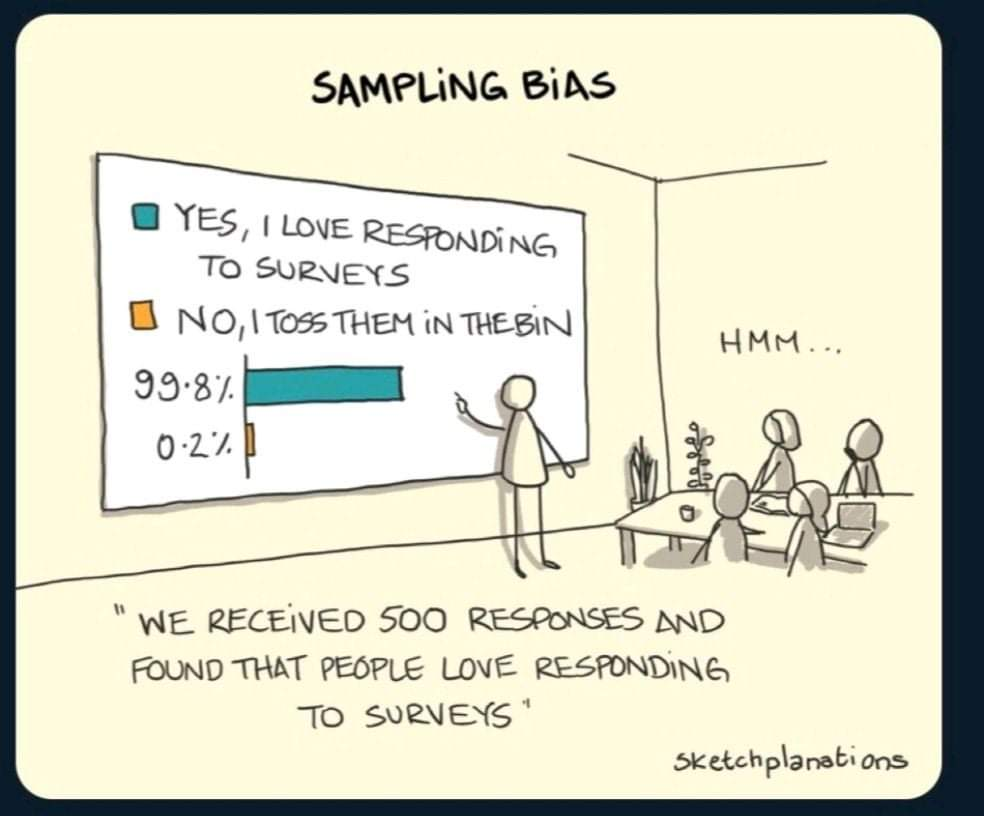
\includegraphics[width=0.42\linewidth,height=\textheight,keepaspectratio]{attachments/samplingBias.jpg}
\end{center}
\end{frame}

\begin{frame}{}
\phantomsection\label{section-5}
Gli strumenti statistici consentono di valutare
\textbf{probabilisticamente} gli errori che si possono commettere
traendo conclusioni sulle popolazioni a partire dalle caratteristiche di
uno o più campioni

\vspace{3mm}

Gli errori di un'indagine campionaria possono essere ridotti se il
campione è \textbf{rappresentativo} della popolazione; dovrebbe cioè
\emph{possedere le caratteristiche della popolazione dalla quale
proviene}

\begin{tcolorbox}[enhanced jigsaw, opacityback=0, bottomtitle=1mm, bottomrule=.15mm, titlerule=0mm, coltitle=black, toprule=.15mm, breakable, toptitle=1mm, colbacktitle=quarto-callout-important-color!10!white, arc=.35mm, title={Campionamento casuale}, rightrule=.15mm, leftrule=.75mm, opacitybacktitle=0.6, left=2mm, colframe=quarto-callout-important-color-frame, colback=white]

Se il campione è estratto \emph{casualmente} dalla popolazione si può
affermare che eventuali differenze sono dovute ``al caso'', dovute cioè
\emph{a variazioni accidentali e non sistematiche}

\end{tcolorbox}
\end{frame}

\begin{frame}{}
\phantomsection\label{section-6}
Non solo come\ldots{} ma anche quanto! L'importanza dell'ampiezza
campionaria per studi che permettano inferenze ``valide''

\begin{center}

\includegraphics[width=0.48\linewidth,height=\textheight,keepaspectratio]{attachments/sampleSize.jpg}
\end{center}
\end{frame}

\section{Stimatore}\label{stimatore}

\begin{frame}{}
\phantomsection\label{section-7}
Un \textbf{indicatore o statistica} o più comunemente \textbf{STIMATORE}
è una funzione dei valori osservati sul campione
\((X_1, X_2, \ldots, X_n)\), utilizzato per la stima di un
\textbf{parametro} (generalmente incognito) di una \textbf{popolazione}
e che (possibilmente) rispetta una serie di caratteristiche.

\vspace{3mm}

Stima:

\begin{itemize}
\tightlist
\item
  \emph{Stima puntuale}: il metodo di stima conduce ad un unico valore
  per il parametro in oggetto
\item
  \emph{Stima intervallare}: il metodo di stima conduce ad un intervallo
  di valori, all'interno dei quali si suppone che si trovi con una certa
  probabilità il valore vero del parametro
\end{itemize}
\end{frame}

\begin{frame}{Proprietà di uno stimatore}
\phantomsection\label{proprietuxe0-di-uno-stimatore}
\footnotesize

Uno stimatore è tanto migliore quanto più rispetta queste proprietà:

\vspace{2mm}

\begin{itemize}
\tightlist
\item
  \textbf{Correttezza} (o non distorsione): in media, su tutti i
  campioni possibili, lo stimatore restituisce il valore del parametro
  \textcolor{evid}{$\rightarrow$} ad es., \(\mu_{\bar{x}} = \mu\)
\end{itemize}

\vspace{1mm}

\begin{itemize}
\tightlist
\item
  \textbf{Efficienza}: tra due stimatori corretti, è più efficiente
  quello con varianza minore \textcolor{evid}{$\rightarrow$} le stime
  cambiano meno da un campione all'altro
\end{itemize}

\vspace{1mm}

\begin{itemize}
\tightlist
\item
  \textbf{Consistenza}: all'aumentare dell'ampiezza campionaria \(n\),
  le stime si avvicinano sempre di più al valore del parametro
\end{itemize}

\vspace{3mm}

La media campionaria \(\bar{x}\) è uno stimatore corretto e consistente
della media della popolazione \(\mu\) (lo si vede nell'esempio sulle
distribuzioni campionarie)
\end{frame}

\begin{frame}{}
\phantomsection\label{section-8}
La \textbf{statistica inferenziale} ha pertanto l'obiettivo di stimare
incogniti parametri attraverso certe funzioni dei dati campionari
(\emph{indicatori} o \emph{stimatori}).

\vspace{3mm}

Si calcolano, quindi, le \textbf{STATISTICHE} (ad es., \(\bar{x}\)) del
campione per conoscere i \textbf{PARAMETRI} (ad es., \(\mu\)) della
popolazione.

\vspace{3mm}

Questo passaggio dalle STATISTICHE ai PARAMETRI si basa sulla conoscenza
delle proprietà delle \textbf{DISTRIBUZIONI CAMPIONARIE} delle
statistiche (ad es., \(M\))
\end{frame}

\section{Distribuzioni campionarie}\label{distribuzioni-campionarie}

\begin{frame}{Distribuzione campionaria}
\phantomsection\label{distribuzione-campionaria}
\small

\begin{quote}
La \textbf{distribuzione campionaria} è la \emph{distribuzione di
probabilità} relativa a una specifica statistica calcolata su tutti i
\(k\) campioni estraibili da una popolazione
\end{quote}

Per determinare una distribuzione campionaria:

\begin{enumerate}
\item
  Estrarre tutti i possibili \(k\) campioni dalla popolazione di
  interesse con campionamento \emph{casuale e indipendente}
  \textcolor{evid}{$\rightarrow$} ogni unità di analisi deve avere la
  stessa probabilità di essere estratta e l'estrazione di una unità non
  deve modificare la probabilità delle altre unità
\item
  Calcolare su ognuno dei \(k\) campioni la statistica di interesse
\item
  Determinare (i.e., contare) la frequenza per ognuno dei valori della
  statistica \textcolor{evid}{$\rightarrow$} quanti \emph{campioni}
  presentano quel valore
\end{enumerate}
\end{frame}

\subsection{Distribuzione campionaria della
media}\label{distribuzione-campionaria-della-media}

\begin{frame}{}
\phantomsection\label{section-9}
\begin{center}
\begin{tikzpicture}[scale=0.8, every node/.style={transform shape}]
  \node (a) [type1, xshift=-3cm] {};
  \node (b) [type2, right of=a, xshift=0.5cm]{};
  \node (c) [type3, right of=b, xshift=0.5cm]{};
  \node (d) [type4, right of=c, xshift=0.5cm]{};
  \node (e) [type5, right of=d, xshift=0.5cm]{};
  \node (f) [type6, right of=e, xshift=0.5cm]{};
  \node (pop)[info, right of =f , xshift=1.5cm] {Popolazione};
  \onslide<2->
  \node[draw=red,fit=(a) (b) ,inner sep=0.8ex,ellipse] (c1) {};
  \node[draw=black,fit=(b) (c) ,inner sep=0.5ex,ellipse] (c2) {};
  \node[draw=blue,fit=(c) (d) ,inner sep=0.8ex,ellipse] (c3) {};
  \node[draw=cyan,fit=(d) (e) ,inner sep=0.5ex,ellipse] (c4) {};
  \node[draw=olive,fit=(e) (f) ,inner sep=0.8ex,ellipse] (c5) {};

  \node (g1a) [type1,below of=c1, xshift=-0.8cm, yshift=-0.5cm] {};
  \node (g1b) [type2,right of=g1a, xshift=-0.3cm] {};
  \node[draw = black, fit = (g1a) (g1b), rectangle] (g1) {};

  \node (g2a) [type2,right of=g1b, xshift=0.15cm] {};
  \node (g2b) [type3,right of=g2a, xshift=-0.3cm] {};
  \node[draw = black, fit = (g2a) (g2b), rectangle] (g2) {};

  \node (g3a) [type3,right of=g2b, xshift=0.15cm] {};
  \node (g3b) [type4,right of=g3a, xshift=-0.3cm] {};
  \node[draw = black, fit = (g3a) (g3b), rectangle] (g3) {};

  \node (g4a) [type4,right of=g3b, xshift=0.15cm] {};
  \node (g4b) [type5,right of=g4a, xshift=-0.3cm] {};
  \node[draw = black, fit = (g4a) (g4b), rectangle] (g4) {};

  \node (g5a) [type5,right of=g4b, xshift=0.15cm] {};
  \node (g5b) [type6,right of=g5a, xshift=-0.3cm] {};
  \node[draw = black, fit = (g5a) (g5b), rectangle] (g5) {};

  \node (campione) [info, right of=g5, xshift=1.5cm] {Campione};

  \draw[thick,->,>=stealth, red] (c1) edge (g1);
  \draw[thick,->,>=stealth, black] (c2) edge (g2);
  \draw[thick,->,>=stealth, blue] (c3) edge (g3);
  \draw[thick,->,>=stealth, cyan] (c4) edge (g4);
  \draw[thick,->,>=stealth, giallo] (c5) edge (g5);
  \onslide<3->
  \node (m1) [stat, below of= g1, yshift=-1cm] {\color{red}$M_1$};
  \node (m2) [stat, below of= g2, yshift=-1cm] {\color{black}$M_2$};
  \node (m3) [stat, below of= g3, yshift=-1cm] {\color{blue}$\ldots$};
  \node (m4) [stat, below of= g4, yshift=-1cm] {\color{cyan}$\ldots$};
  \node (m5) [stat, below of= g5, yshift=-1cm] {\color{giallo}$M_5$};

  \draw[thick,->,>=stealth] (g1) edge (m1);
  \draw[thick,->,>=stealth] (g2) edge (m2);
  \draw[thick,->,>=stealth] (g3) edge (m3);
  \draw[thick,->,>=stealth] (g4) edge (m4);
  \draw[thick,->,>=stealth] (g5) edge (m5);

  \node (statistica) [info, right of= m5, xshift = 1cm] {Statistica};

  \onslide<4->
  \node (mediaGen) [info, below of= m3, yshift= -1cm] {$\mu_{\bar{X}} = \frac{M_1 + M_2 + \ldots + M_k}{k}$};
  \node (dcm) [info, below of= statistica, yshift= -1cm] {Distribuzione campionaria della media};

  \draw[thick,->,>=stealth] (m1) edge (mediaGen);
  \draw[thick,->,>=stealth] (m2) edge (mediaGen);
  \draw[thick,->,>=stealth] (m3) edge (mediaGen);
  \draw[thick,->,>=stealth] (m4) edge (mediaGen);
  \draw[thick,->,>=stealth] (m5) edge (mediaGen);
\end{tikzpicture}
\end{center}

\uncover<2->{\footnotesize \textcolor{unipd}{\textbf{N.B.:}} Sono illustrati solo alcuni dei possibili $k$ campioni}
\end{frame}

\begin{frame}{Esempio}
\phantomsection\label{esempio-1}
Popolazione: \(N = 5\) \newline Campione: \(n = 2\), somministrato un
test con punteggio 0--10

\vspace{2mm}

\begin{columns}[T]
\begin{column}{0.36\linewidth}
\centering

\textbf{Popolazione} \(N = 5\)

\small

\begin{longtable}[]{@{}lc@{}}
\toprule\noalign{}
Soggetto & Punteggio \\
\midrule\noalign{}
\endhead
Giorgio & 6 \\
Alessandra & 8 \\
Francesco & 10 \\
Livio & 3 \\
Jessica & 8 \\
\bottomrule\noalign{}
\end{longtable}

\[\mu = \dfrac{6 + 8 + 10 + 3 + 8}{5} = 7\]
\end{column}

\begin{column}{0.32\linewidth}
\centering

\textbf{Campione} \(n = 2\)

\small

\begin{longtable}[]{@{}lc@{}}
\toprule\noalign{}
Soggetto & Punteggio \\
\midrule\noalign{}
\endhead
Giorgio & 6 \\
Alessandra & 8 \\
\bottomrule\noalign{}
\end{longtable}

\[\bar{X} = \dfrac{6 + 8}{2} = 7\]
\end{column}

\begin{column}{0.32\linewidth}
\centering

E un altro campione?

\small

\begin{longtable}[]{@{}lc@{}}
\toprule\noalign{}
Soggetto & Punteggio \\
\midrule\noalign{}
\endhead
Alessandra & 8 \\
Francesco & 10 \\
\bottomrule\noalign{}
\end{longtable}

\[\bar{X} = \dfrac{8 + 10}{2} = 9\]
\end{column}
\end{columns}
\end{frame}

\begin{frame}{Tutti i campioni possibili}
\phantomsection\label{tutti-i-campioni-possibili}
\begin{center}
\scalebox{.50}{
  \begin{tabular}{c|ccc ca|c|c ccca}
    \hline
    Campione & Elemento 1 & Elemento 2 & Valore 1 & Valore 2 & \textbf{Media} & Campione & Elemento 1 & Elemento 2 & Valore 1 & Valore 2 & \textbf{Media} \\\hline
    1  & G & G & 6  & 6  & 6   & 16 & L & G & 3 & 6  & 4.5 \\
    2  & G & A & 6  & 8  & 7   & 17 & L & A & 3 & 8  & 5.5 \\
    3  & G & F & 6  & 10 & 8   & 18 & L & F & 3 & 10 & 6.5 \\
    4  & G & L & 6  & 3  & 4.5 & 19 & L & L & 3 & 3  & 3   \\
    5  & G & J & 6  & 8  & 7   & 20 & L & J & 3 & 8  & 5.5 \\
    6  & A & G & 8  & 6  & 7   & 21 & J & G & 8 & 6  & 7   \\
    7  & A & A & 8  & 8  & 8   & 22 & J & A & 8 & 8  & 8   \\
    8  & A & F & 8  & 10 & 9   & 23 & J & F & 8 & 10 & 9   \\
    9  & A & L & 8  & 3  & 5.5 & 24 & J & L & 8 & 3  & 5.5 \\
    10 & A & J & 8  & 8  & 8   & 25 & J & J & 8 & 8  & 8   \\
    11 & F & G & 10 & 6  & 8   &    &   &   &   &    &     \\
    12 & F & A & 10 & 8  & 9   &    &   &   &   &    &     \\
    13 & F & F & 10 & 10 & 10  &    &   &   &   &    &     \\
    14 & F & L & 10 & 3  & 6.5 &    &   &   &   &    &     \\
    15 & F & J & 10 & 8  & 9   &    &   &   &   &    &     \\
    \hline
  \end{tabular}
}
\end{center}

\footnotesize

\[\mu_{\bar{x}} = \dfrac{6 \cdot 1 + 7 \cdot 4 + 8 \cdot 6 + 4.5 \cdot 2 + 9 \cdot 4 + 5.5 \cdot 4 + 10 \cdot 1 + 6.5 \cdot 2 + 3 \cdot 1}{25} = 7\]

\[\mu = \mu_{\bar{x}} = 7\]
\end{frame}

\begin{frame}{La distribuzione campionaria dell'esempio}
\phantomsection\label{la-distribuzione-campionaria-dellesempio}
\small

Frequenza di ciascun valore della media sui 25 campioni possibili (passo
3 della definizione):

\begin{center}
\begin{tikzpicture}[xscale=1, yscale=0.9]
  \draw[->] (-0.5,0) -- (7.6,0) node[right, font=\scriptsize] {$\bar{x}$};
  \draw[->] (-0.5,0) -- (-0.5,3.4) node[above, font=\scriptsize] {Frequenza};
  \fill[evid!60] (-0.20,0) rectangle (0.20,0.5);
  \node[above, font=\scriptsize] at (0.00,0.5) {1};
  \node[below, font=\scriptsize] at (0.00,0) {3};
  \fill[evid!60] (1.30,0) rectangle (1.70,1.0);
  \node[above, font=\scriptsize] at (1.50,1.0) {2};
  \node[below, font=\scriptsize] at (1.50,0) {4.5};
  \fill[evid!60] (2.30,0) rectangle (2.70,2.0);
  \node[above, font=\scriptsize] at (2.50,2.0) {4};
  \node[below, font=\scriptsize] at (2.50,0) {5.5};
  \fill[evid!60] (2.80,0) rectangle (3.20,0.5);
  \node[above, font=\scriptsize] at (3.00,0.5) {1};
  \node[below, font=\scriptsize] at (3.00,0) {6};
  \fill[evid!60] (3.30,0) rectangle (3.70,1.0);
  \node[above, font=\scriptsize] at (3.50,1.0) {2};
  \node[below, font=\scriptsize] at (3.50,0) {6.5};
  \fill[evid!60] (3.80,0) rectangle (4.20,2.0);
  \node[above, font=\scriptsize] at (4.00,2.0) {4};
  \node[below, font=\scriptsize] at (4.00,0) {7};
  \fill[evid!60] (4.80,0) rectangle (5.20,3.0);
  \node[above, font=\scriptsize] at (5.00,3.0) {6};
  \node[below, font=\scriptsize] at (5.00,0) {8};
  \fill[evid!60] (5.80,0) rectangle (6.20,2.0);
  \node[above, font=\scriptsize] at (6.00,2.0) {4};
  \node[below, font=\scriptsize] at (6.00,0) {9};
  \fill[evid!60] (6.80,0) rectangle (7.20,0.5);
  \node[above, font=\scriptsize] at (7.00,0.5) {1};
  \node[below, font=\scriptsize] at (7.00,0) {10};
  \draw[dashed, unipd, thick] (4,0) -- (4,3.3) node[above, font=\scriptsize] {$\mu = 7$};
\end{tikzpicture}
\end{center}

Le medie campionarie si distribuiscono \textbf{attorno a \(\mu = 7\)}:
alcuni campioni sovrastimano \(\mu\), altri lo sottostimano, ma in media
lo stimatore restituisce il valore del parametro (correttezza)
\end{frame}

\begin{frame}{Errore standard}
\phantomsection\label{errore-standard}
\footnotesize

Oltre al centro della distribuzione campionaria serve sapere
\textbf{quanto variano} le medie da un campione all'altro

\begin{tcolorbox}[enhanced jigsaw, opacityback=0, bottomtitle=1mm, bottomrule=.15mm, titlerule=0mm, coltitle=black, toprule=.15mm, breakable, toptitle=1mm, colbacktitle=quarto-callout-tip-color!10!white, arc=.35mm, title={Errore standard della media}, rightrule=.15mm, leftrule=.75mm, opacitybacktitle=0.6, left=2mm, colframe=quarto-callout-tip-color-frame, colback=white]

È la deviazione standard della distribuzione campionaria della media:
\[\sigma_{\bar{x}} = \frac{\sigma}{\sqrt{n}}\] dove \(\sigma\) è la
deviazione standard della popolazione e \(n\) l'ampiezza dei campioni

\end{tcolorbox}

Nell'esempio: \(\sigma^2 = 5.6\) (varianza della popolazione), mentre la
varianza delle 25 medie è \(2.8 = \frac{5.6}{2}\), quindi
\(\sigma_{\bar{x}} = \frac{\sqrt{5.6}}{\sqrt{2}} = 1.67\)

\vspace{2mm}

All'aumentare di \(n\) l'errore standard diminuisce
\textcolor{evid}{$\rightarrow$} con campioni più grandi la media
campionaria è una stima più precisa di \(\mu\) (consistenza)
\end{frame}

\begin{frame}{Forma della distribuzione campionaria}
\phantomsection\label{forma-della-distribuzione-campionaria}
\footnotesize

\begin{tcolorbox}[enhanced jigsaw, opacityback=0, bottomtitle=1mm, bottomrule=.15mm, titlerule=0mm, coltitle=black, toprule=.15mm, breakable, toptitle=1mm, colbacktitle=quarto-callout-important-color!10!white, arc=.35mm, title={Teorema del limite centrale}, rightrule=.15mm, leftrule=.75mm, opacitybacktitle=0.6, left=2mm, colframe=quarto-callout-important-color-frame, colback=white]

Se l'ampiezza campionaria \(n\) è sufficientemente grande (regola
pratica: \(n \geq 30\)), la distribuzione campionaria della media è
\textbf{approssimativamente normale}, con media \(\mu\) e deviazione
standard \(\frac{\sigma}{\sqrt{n}}\), \emph{qualunque sia la forma della
distribuzione nella popolazione}

\end{tcolorbox}

Se la popolazione ha distribuzione normale, la distribuzione campionaria
della media è normale per qualsiasi \(n\)

\vspace{2mm}

Standardizzando la media campionaria si ottiene una variabile normale
standard: \[z = \frac{\bar{x} - \mu}{\sigma / \sqrt{n}} \sim N(0, 1)\]

È questa la \textbf{curva} su cui si costruiscono le regioni di rifiuto
e di non rifiuto del test di ipotesi
\end{frame}

\section{Test di ipotesi}\label{test-di-ipotesi}

\begin{frame}{}
\phantomsection\label{section-10}
Obiettivi dell'inferenza statistica:

\begin{itemize}
\tightlist
\item
  Stima dei parametri
\item
  \textbf{Test di ipotesi}
\end{itemize}

\begin{center}

\includegraphics[width=0.06\linewidth,height=\textheight,keepaspectratio]{frecciadown.png}
\end{center}

Procedura che si svolge per passi logici successivi:

\begin{itemize}
\tightlist
\item
  (Porsi una domanda di ricerca) (dotata di senso) (basata sulla
  letteratura)
\item
  Formulazione ipotesi riguardanti i parametri della popolazione
\item
  Definizione dei criteri e dei vincoli di accettazione dell'ipotesi
\item
  Raccolta dati campionari
\item
  Valutazione delle ipotesi formulate
\end{itemize}
\end{frame}

\begin{frame}{}
\phantomsection\label{section-11}
\small

Le ipotesi di ricerca sono ipotesi statistiche:

\begin{itemize}
\tightlist
\item
  consistono in affermazioni di tipo logico-matematico che definiscono i
  rapporti fra i parametri di una o più popolazioni
\item
  il test delle ipotesi consiste in un \textbf{processo di decisione che
  termina nell'accettazione --o non rifiuto-- delle affermazioni
  contenute nelle ipotesi stesse}
\item
  Un'ipotesi statistica è un'asserzione o supposizione sulla
  distribuzione di una o più variabili casuali, o su uno o più parametri
  della stessa, e si indica con la lettera \textbf{\emph{H}}.
\end{itemize}

\begin{tcolorbox}[enhanced jigsaw, opacityback=0, bottomtitle=1mm, bottomrule=.15mm, titlerule=0mm, coltitle=black, toprule=.15mm, breakable, toptitle=1mm, colbacktitle=quarto-callout-note-color!10!white, arc=.35mm, title={Esempio}, rightrule=.15mm, leftrule=.75mm, opacitybacktitle=0.6, left=2mm, colframe=quarto-callout-note-color-frame, colback=white]

Sia \(X_1, X_2, \ldots, X_n\) un campione casuale estratto da una
popolazione normale con media incognita. Si può formulare l'ipotesi che
la media di tale popolazione sia 12. Formalmente si esprime con:
\[\text{H}:\; \mu = 12\]

\end{tcolorbox}
\end{frame}

\subsection{Null Hypothesis Significance Testing
(NHST)}\label{null-hypothesis-significance-testing-nhst}

\begin{frame}{Due approcci\ldots{} e un ibrido}
\phantomsection\label{due-approcci-e-un-ibrido}
\small

\begin{columns}[T]
\begin{column}{0.5\linewidth}
\textbf{Fisher (1925)}

\begin{itemize}
\tightlist
\item
  Solo \(H_0\), nessuna ipotesi alternativa formale
\item
  Il \(p\)-value indica quanto i dati sono poco compatibili con \(H_0\)
\end{itemize}
\end{column}

\begin{column}{0.5\linewidth}
\textbf{Neyman e Pearson (1933)}

\begin{itemize}
\tightlist
\item
  \(H_0\) contro \(H_1\)
\item
  \(\alpha\) e \(\beta\) fissati prima di raccogliere i dati
  \(\rightarrow\) decisione: si rifiuta o non si rifiuta \(H_0\)
\end{itemize}
\end{column}
\end{columns}

\vspace{3mm}

\begin{tcolorbox}[enhanced jigsaw, opacityback=0, bottomtitle=1mm, bottomrule=.15mm, titlerule=0mm, coltitle=black, toprule=.15mm, breakable, toptitle=1mm, colbacktitle=quarto-callout-important-color!10!white, arc=.35mm, title={NHST}, rightrule=.15mm, leftrule=.75mm, opacitybacktitle=0.6, left=2mm, colframe=quarto-callout-important-color-frame, colback=white]

È una \emph{forzatura} dei due approcci: prende \(H_0\) e il \(p\)-value
da Fisher, \(H_1\), \(\alpha\) e \(\beta\) da Neyman e Pearson, e li
mette insieme (anche se i due approcci hanno logiche diverse)

\end{tcolorbox}
\end{frame}

\begin{frame}{}
\phantomsection\label{section-12}
\small

\begin{tcolorbox}[enhanced jigsaw, opacityback=0, bottomtitle=1mm, bottomrule=.15mm, titlerule=0mm, coltitle=black, toprule=.15mm, breakable, toptitle=1mm, colbacktitle=quarto-callout-tip-color!10!white, arc=.35mm, title={Ipotesi nulla e ipotesi alternativa}, rightrule=.15mm, leftrule=.75mm, opacitybacktitle=0.6, left=2mm, colframe=quarto-callout-tip-color-frame, colback=white]

Le distribuzioni di probabilità a livello delle popolazioni che
identificano lo schema logico del confronto sono classificate in due
gruppi distinti:

\begin{itemize}
\tightlist
\item
  \textbf{H\(_0\)}: definita come \textbf{l'ipotesi nulla}
\item
  \textbf{H\(_A\)}: definita come \textbf{l'ipotesi alternativa}
\end{itemize}

L'ipotesi alternativa viene indicata con altri simboli equivalenti come
\textbf{H\(_1\)} oppure \textbf{K}, che sono di fatto sinonimi del più
diffuso H\(_A\).

\end{tcolorbox}

\begin{tcolorbox}[enhanced jigsaw, opacityback=0, bottomtitle=1mm, bottomrule=.15mm, titlerule=0mm, coltitle=black, toprule=.15mm, breakable, toptitle=1mm, colbacktitle=quarto-callout-warning-color!10!white, arc=.35mm, title={Nota}, rightrule=.15mm, leftrule=.75mm, opacitybacktitle=0.6, left=2mm, colframe=quarto-callout-warning-color-frame, colback=white]

H\(_0\) è definita come la \textbf{negazione logica} di H\(_A\) e
viceversa.

Ad esempio, supponiamo che H\(_0\) affermi che \(\mu \leq \mu_0\),
allora H\(_A\) indica la relazione complementare \(\mu > \mu_0\).
\[\Theta_0 = (\Theta_A)^c\]

\end{tcolorbox}
\end{frame}

\begin{frame}{}
\phantomsection\label{section-13}
\begin{enumerate}
\tightlist
\item
  \textbf{Ipotesi \(H_0\)}: è l'ipotesi che costituisce l'oggetto del
  test; specifica i valori dei parametri della popolazione da cui si
  suppone provenga il campione (o i campioni) in esame. Stabilisce che i
  diversi valori ottenuti nel campione sono puramente \textbf{casuali}.
  Formalmente si esprime con: \[H_0: \; \theta = \theta_0\] dove
  \(\theta\) indica il parametro della popolazione e \(\theta_0\) il
  valore che ci si attende
\end{enumerate}

\begin{center}
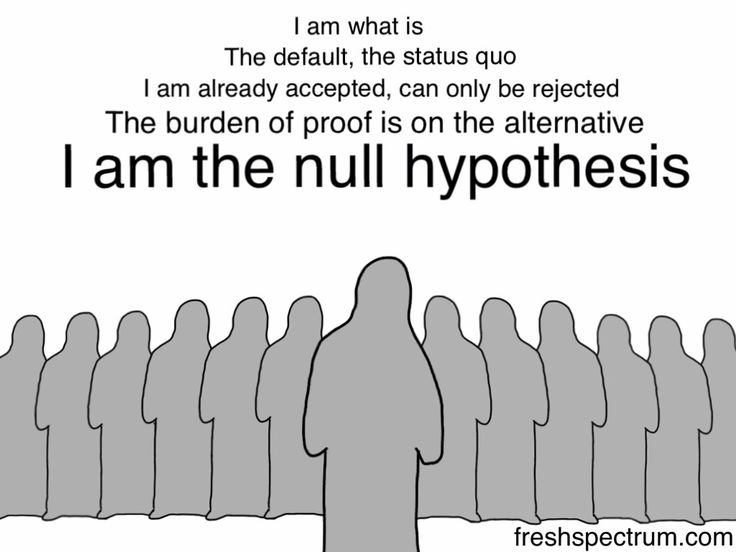
\includegraphics[width=0.4\linewidth,height=\textheight,keepaspectratio]{nhst.jpg}
\end{center}
\end{frame}

\begin{frame}{}
\phantomsection\label{section-14}
\begin{enumerate}
\setcounter{enumi}{1}
\tightlist
\item
  \textbf{Ipotesi \(H_1\)}: è l'ipotesi alternativa, solitamente
  l'ipotesi di ricerca secondo la quale i risultati ottenuti \textbf{non
  sono casuali} ma sono spiegabili secondo una qualche regola o teoria.
  L'ipotesi alternativa può essere:
\end{enumerate}

\vspace{1.5mm}

\begin{center}
\Large \textbf{Bidirezionale}

\vspace{1.5mm}

\colorbox{evid!20}{$\theta \neq \theta_0$}
\end{center}

\vspace{1.5mm}

\begin{center}
\Large \textbf{Monodirezionale}
\end{center}

\begin{columns}[T]
\begin{column}{0.5\linewidth}
\centering
\Large

\textbf{Sinistra}

\colorbox{giallo!40}{$\theta < \theta_0$}
\end{column}

\begin{column}{0.5\linewidth}
\centering
\Large

\textbf{Destra}

\colorbox{olive!20}{$\theta > \theta_0$}
\end{column}
\end{columns}
\end{frame}

\begin{frame}{}
\phantomsection\label{section-15}
\begin{tcolorbox}[enhanced jigsaw, opacityback=0, bottomtitle=1mm, bottomrule=.15mm, titlerule=0mm, coltitle=black, toprule=.15mm, breakable, toptitle=1mm, colbacktitle=quarto-callout-note-color!10!white, arc=.35mm, title={Esempio}, rightrule=.15mm, leftrule=.75mm, opacitybacktitle=0.6, left=2mm, colframe=quarto-callout-note-color-frame, colback=white]

Si vuole stabilire, attraverso un esperimento, se una moneta sia
truccata o meno. Si indicherà con \(\pi\) la probabilità di ottenere
testa in un lancio. Prima di eseguire l'esperimento si devono formulare
le due ipotesi relativamente al parametro \(\pi\):

\vspace{3mm}

\begin{itemize}
\tightlist
\item
  \(H_0: \; \pi = .50\) la moneta non è truccata
\end{itemize}

\vspace{3mm}

\begin{itemize}
\tightlist
\item
  \(H_1: \; \pi \neq .50\) la moneta è truccata
\end{itemize}

\end{tcolorbox}
\end{frame}

\begin{frame}{}
\phantomsection\label{section-16}
Il problema è stabilire se i risultati dell'esperimento (ad es. lanciare
una moneta 30 volte) falsificano o meno l'ipotesi;

\vspace{3mm}

I valori empirici possono considerarsi dovuti a fluttuazioni casuali
intorno al valore atteso e di conseguenza non confutare \(H_0\)?

\vspace{3mm}

Oppure il risultato non lo consente, le fluttuazioni non sono casuali ma
sistematiche e di conseguenza \(H_0\) è confutata?
\end{frame}

\begin{frame}{}
\phantomsection\label{section-17}
La decisione si basa sul calcolo di un test statistico e sulla
probabilità associata al valore di tale test:

\begin{tcolorbox}[enhanced jigsaw, opacityback=0, bottomtitle=1mm, bottomrule=.15mm, titlerule=0mm, coltitle=black, toprule=.15mm, breakable, toptitle=1mm, colbacktitle=quarto-callout-tip-color!10!white, arc=.35mm, title={Test statistico}, rightrule=.15mm, leftrule=.75mm, opacitybacktitle=0.6, left=2mm, colframe=quarto-callout-tip-color-frame, colback=white]

Valore di una variabile casuale che può assumere i valori di una
distribuzione campionaria caratterizzata da una determinata
distribuzione di probabilità

\end{tcolorbox}

Ogni test statistico divide lo spazio campionario:

\begin{enumerate}
\tightlist
\item
  Regione di non rifiuto di \(H_0\)
\item
  Regione di rifiuto di \(H_0\)
\end{enumerate}

In base alla regione in cui andrà a cadere il valore campionario, si
prenderà una decisione sull'ipotesi \(H_0\)
\end{frame}

\begin{frame}{}
\phantomsection\label{section-18}
Le regioni di rifiuto e di accettazione corrispondono ad aree di
probabilità sottese alla curva

\begin{center}
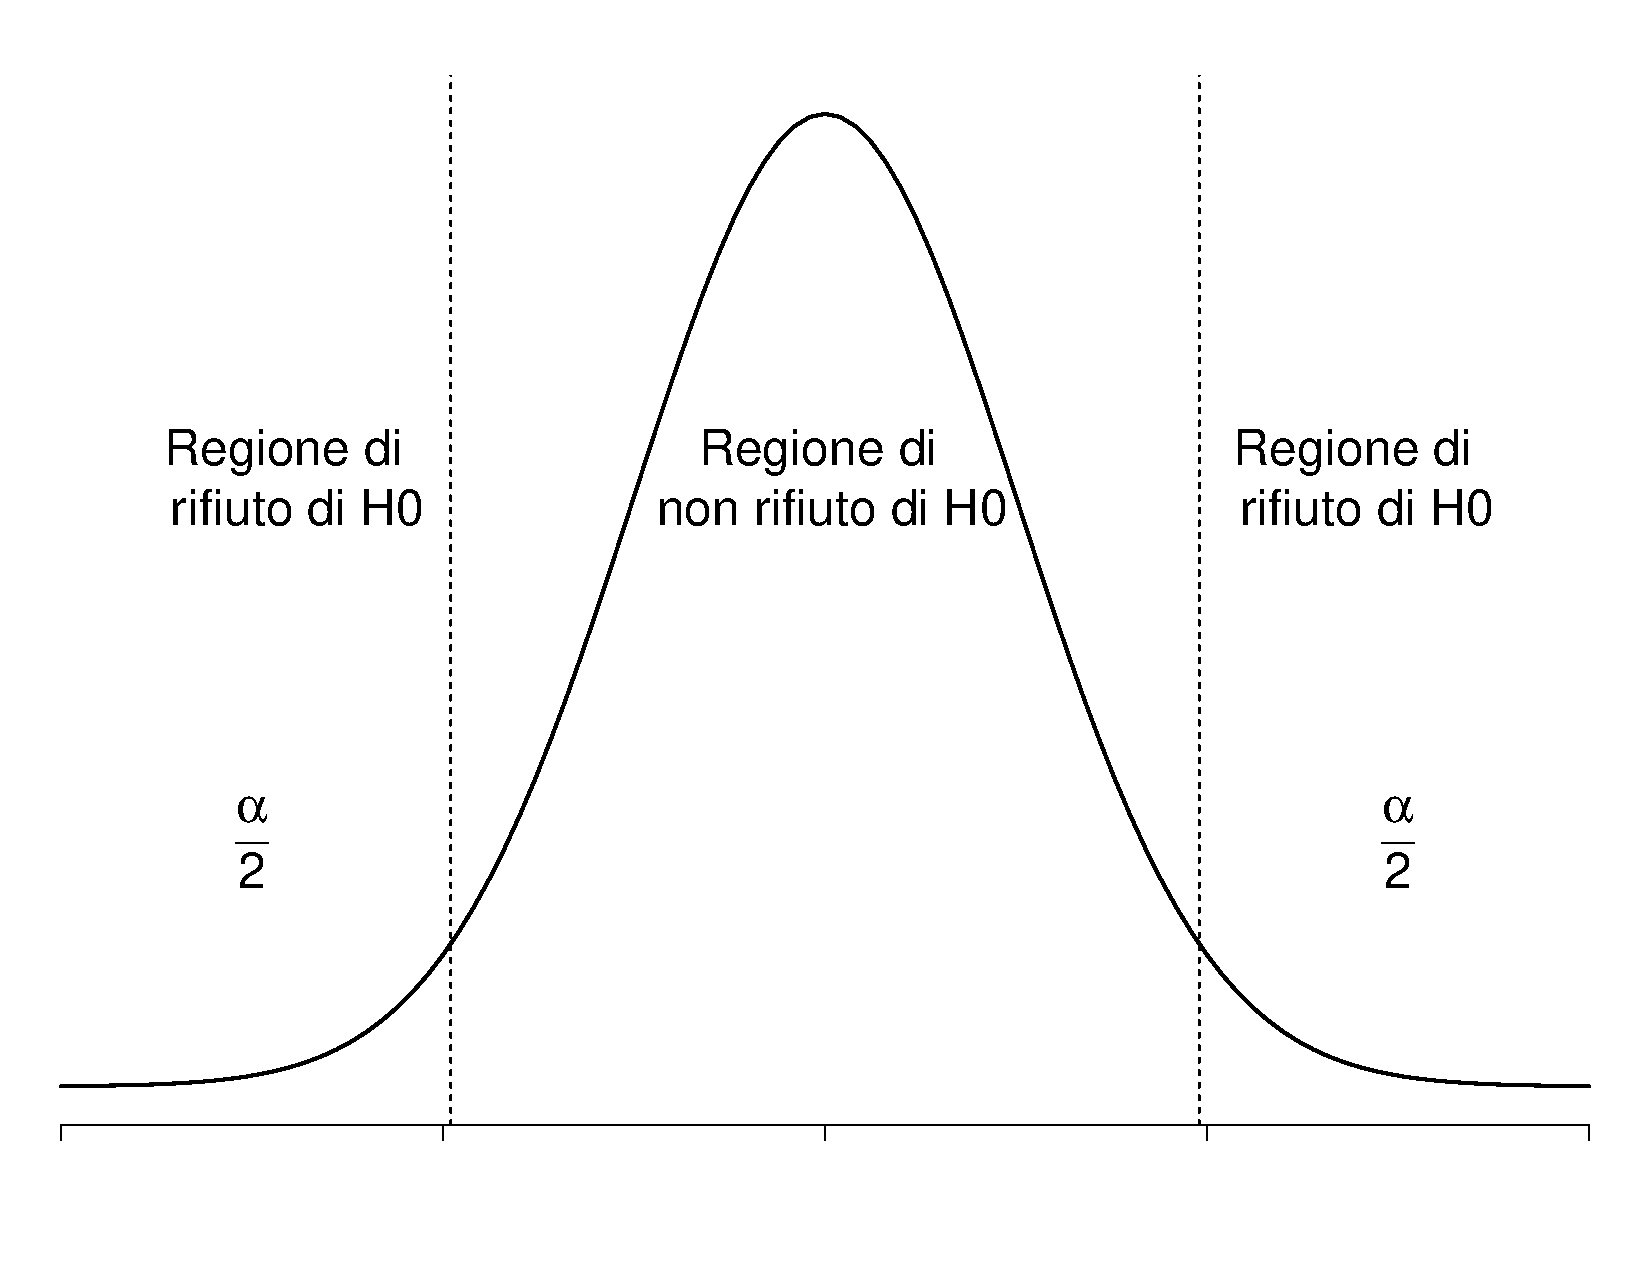
\includegraphics[width=0.45\linewidth,height=\textheight,keepaspectratio]{regioneRifiutobi.pdf}
\end{center}

\vspace{-1.5mm}

\begin{columns}[T]
\begin{column}{0.5\linewidth}
\small

\textbf{Regione di non rifiuto}: valori delle statistiche campionarie
con probabilità maggiori di verificarsi
\end{column}

\begin{column}{0.5\linewidth}
\small

\textbf{Regione di rifiuto}: valori delle statistiche campionarie con
probabilità molto basse di verificarsi
\end{column}
\end{columns}
\end{frame}

\section{Valore critico}\label{valore-critico}

\begin{frame}{Livello di significatività}
\phantomsection\label{livello-di-significativituxe0}
\small

\begin{tcolorbox}[enhanced jigsaw, opacityback=0, bottomtitle=1mm, bottomrule=.15mm, titlerule=0mm, coltitle=black, toprule=.15mm, breakable, toptitle=1mm, colbacktitle=quarto-callout-tip-color!10!white, arc=.35mm, title={\(\alpha\)}, rightrule=.15mm, leftrule=.75mm, opacitybacktitle=0.6, left=2mm, colframe=quarto-callout-tip-color-frame, colback=white]

Il \textbf{livello di significatività} \(\alpha\) è la probabilità di
rifiutare \(H_0\) quando \(H_0\) è vera. Si fissa \textbf{prima} di
raccogliere i dati (valori convenzionali: \(.05\), \(.01\))

\end{tcolorbox}

\vspace{2mm}

\begin{itemize}
\tightlist
\item
  \(\alpha\) è l'area della \textbf{regione di rifiuto} sotto la
  distribuzione campionaria costruita assumendo vera \(H_0\)
\item
  \(1 - \alpha\) è l'area della \textbf{regione di non rifiuto}
\end{itemize}

\vspace{2mm}

Una volta scelto \(\alpha\), la regione di rifiuto è fissata e con essa
il \textbf{valore critico}
\end{frame}

\begin{frame}{}
\phantomsection\label{section-19}
\small

È il valore che separa le due regioni

\vspace{1.5mm}

Per stabilire se il valore di un test è coerente o meno con l'ipotesi
nulla è necessario verificare che il suo valore sia compreso all'interno
della \textbf{regione di non rifiuto}.

\vspace{1.5mm}

Se il valore campionario cade nella \textbf{regione di rifiuto} c'è da
ritenere che le osservazioni campionarie si discostino dai valori più
probabili della distribuzione; in tal caso si può decidere di rifiutare
\(H_0\).
\end{frame}

\begin{frame}[fragile]{Valore critico e direzione di \(H_1\)}
\phantomsection\label{valore-critico-e-direzione-di-h_1}
\small

La posizione della regione di rifiuto dipende da \(H_1\). Esempio con la
normale standard e \(\alpha = .05\):

\begin{center}
\begin{tikzpicture}[scale=0.55]
  \begin{scope}[xshift=0cm]
    \fill[unipd!35] (-3.3,0) -- plot[domain=-3.3:-1.96,samples=60] (\x,{2.2*exp(-\x*\x/2)}) -- (-1.96,0) -- cycle;
    \fill[unipd!35] (1.96,0) -- plot[domain=1.96:3.3,samples=60] (\x,{2.2*exp(-\x*\x/2)}) -- (3.3,0) -- cycle;
    \draw[thick] plot[domain=-3.3:3.3,samples=60] (\x,{2.2*exp(-\x*\x/2)});
    \draw (-3.3,0) -- (3.3,0);
    \draw[dashed] (-1.96,0) -- (-1.96,2.4);
    \node[below, font=\scriptsize] at (-1.96,0) {$-1.96$};
    \draw[dashed] (1.96,0) -- (1.96,2.4);
    \node[below, font=\scriptsize] at (1.96,0) {$1.96$};
    \node[font=\footnotesize\bfseries] at (0,3) {Bidirezionale: $\theta \neq \theta_0$};
  \end{scope}
  \begin{scope}[xshift=7.5cm]
    \fill[unipd!35] (-3.3,0) -- plot[domain=-3.3:-1.645,samples=60] (\x,{2.2*exp(-\x*\x/2)}) -- (-1.645,0) -- cycle;
    \draw[thick] plot[domain=-3.3:3.3,samples=60] (\x,{2.2*exp(-\x*\x/2)});
    \draw (-3.3,0) -- (3.3,0);
    \draw[dashed] (-1.645,0) -- (-1.645,2.4);
    \node[below, font=\scriptsize] at (-1.645,0) {$-1.645$};
    \node[font=\footnotesize\bfseries] at (0,3) {Sinistra: $\theta < \theta_0$};
  \end{scope}
  \begin{scope}[xshift=15cm]
    \fill[unipd!35] (1.645,0) -- plot[domain=1.645:3.3,samples=60] (\x,{2.2*exp(-\x*\x/2)}) -- (3.3,0) -- cycle;
    \draw[thick] plot[domain=-3.3:3.3,samples=60] (\x,{2.2*exp(-\x*\x/2)});
    \draw (-3.3,0) -- (3.3,0);
    \draw[dashed] (1.645,0) -- (1.645,2.4);
    \node[below, font=\scriptsize] at (1.645,0) {$1.645$};
    \node[font=\footnotesize\bfseries] at (0,3) {Destra: $\theta > \theta_0$};
  \end{scope}
\end{tikzpicture}
\end{center}

\vspace{-1mm}

\begin{columns}[T]
\begin{column}{0.33\linewidth}
\centering
\footnotesize

\(\alpha/2 = .025\) in ciascuna coda

\texttt{qnorm(.975)} \(= 1.96\)
\end{column}

\begin{column}{0.33\linewidth}
\centering
\footnotesize

\(\alpha = .05\) nella coda sinistra

\texttt{qnorm(.05)} \(= -1.645\)
\end{column}

\begin{column}{0.33\linewidth}
\centering
\footnotesize

\(\alpha = .05\) nella coda destra

\texttt{qnorm(.95)} \(= 1.645\)
\end{column}
\end{columns}
\end{frame}

\begin{frame}{}
\phantomsection\label{section-20}
I valori delle statistiche campionarie che cadono nella \textbf{zona di
rifiuto} non sono impossibili se \(H_0\) è vera, ma la loro probabilità
è così bassa (\(\leq \alpha\)) che si accetta il rischio di rifiutare
\(H_0\)

\begin{figure}[H]

{\centering 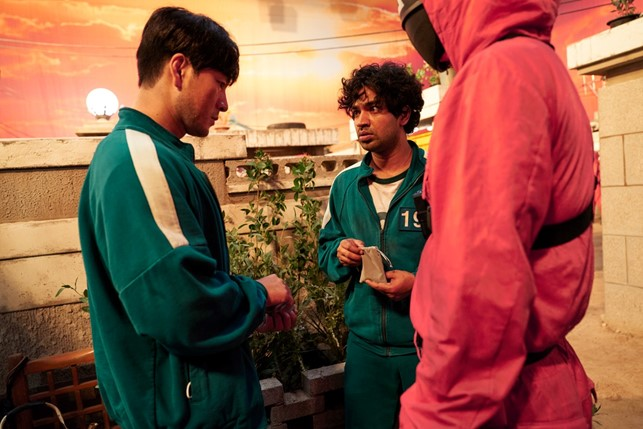
\includegraphics[width=0.6\linewidth,height=\textheight,keepaspectratio]{attachments/squidgame.jpg}

}

\caption{Stai barando vero? Come è possibile che tu vinca a ogni mano??
Le probabilità sono 50-50, vuol dire che stai barando!!!!!}

\end{figure}%
\end{frame}

\begin{frame}{}
\phantomsection\label{section-21}
Una decisione di questo tipo comporta quindi degli errori

\vspace{3mm}

\begin{center}
\renewcommand{\arraystretch}{1.2}
\begin{tabular}{c c |c| c|}
  & \multicolumn{1}{c}{} & \multicolumn{2}{c}{\textcolor{blue}{Ipotesi}} \\
  & \multicolumn{1}{c}{} & \multicolumn{1}{c}{$H_0$ vera} & \multicolumn{1}{c}{$H_0$ falsa} \\
  \cline{3-4}
  \multirow{2}{*}{\textcolor{blue}{Decisione}} & Non si rifiuta $H_0$ & \textcolor{green!10!black!80}{Corretta} & \textcolor{red}{Errata} \\
  \cline{3-4}
  & Si rifiuta $H_0$ & \textcolor{red}{Errata} & \textcolor{green!10!black!80}{Corretta} \\
  \cline{3-4}
\end{tabular}
\end{center}
\end{frame}

\subsection{Errori di I e II tipo}\label{errori-di-i-e-ii-tipo}

\begin{frame}{}
\phantomsection\label{section-22}
\begin{columns}[T]
\begin{column}{0.5\linewidth}
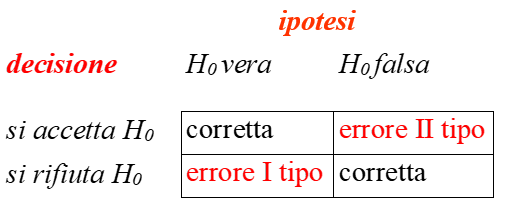
\includegraphics[width=1\linewidth,height=\textheight,keepaspectratio]{Errori.png}
\end{column}

\begin{column}{0.5\linewidth}
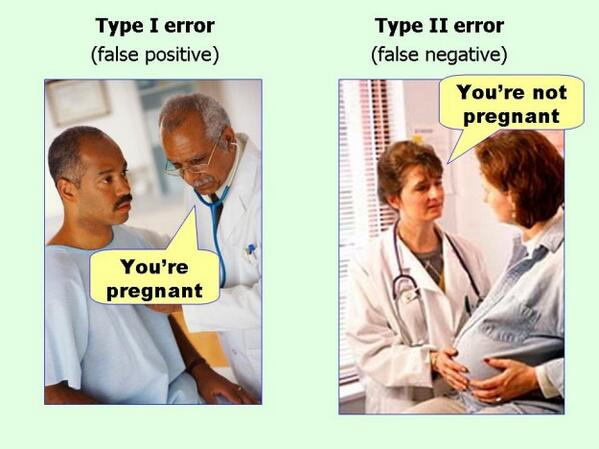
\includegraphics[width=1\linewidth,height=\textheight,keepaspectratio]{pregnant.jpg}
\end{column}
\end{columns}

\vspace{3mm}

Non è mai possibile sapere con certezza se è vera \(H_0\), l'unica cosa
che si può fare è \textbf{minimizzare} la probabilità di prendere una
decisione sbagliata
\end{frame}

\begin{frame}{}
\phantomsection\label{section-23}
\small

La probabilità di non rifiutare \(H_0\) quando è vera è \(1-\alpha\)
(l'area della regione di non rifiuto)

Facendo un ragionamento analogo su \(H_1\) e definendo \(\beta\) la
probabilità di non rifiutare \(H_0\) quando è falsa, si ottiene
\(1- \beta\): la probabilità di rifiutare \(H_0\) quando è falsa, detta
\textbf{potenza} del test

\begin{center}
\renewcommand{\arraystretch}{1.2}
\begin{tabular}{c c |c| c|}
  & \multicolumn{1}{c}{} & \multicolumn{2}{c}{\textcolor{blue}{Ipotesi}} \\
  & \multicolumn{1}{c}{} & \multicolumn{1}{c}{$H_0$ vera} & \multicolumn{1}{c}{$H_0$ falsa} \\
  \cline{3-4}
  \multirow{2}{*}{\textcolor{blue}{Decisione}} & Non si rifiuta $H_0$ & \textcolor{green!10!black!80}{Corretta} ($1-\alpha$) & \textcolor{red}{Errore di II tipo} ($\beta$) \\
  \cline{3-4}
  & Si rifiuta $H_0$ & \textcolor{red}{Errore di I tipo} ($\alpha$) & \textcolor{green!10!black!80}{Corretta} ($1-\beta$) \\
  \cline{3-4}
\end{tabular}
\end{center}

\vspace{3mm}

Quello che si controlla: \(\alpha\) (la probabilità di commettere un
errore di I tipo)

Quello che viene ignorato: \(\beta\) (la probabilità di commettere un
errore di II tipo)
\end{frame}

\begin{frame}{Relazione tra \(\alpha\) e \(\beta\)}
\phantomsection\label{relazione-tra-alpha-e-beta}
\begin{columns}[T]
\begin{column}{0.7\linewidth}
\centering
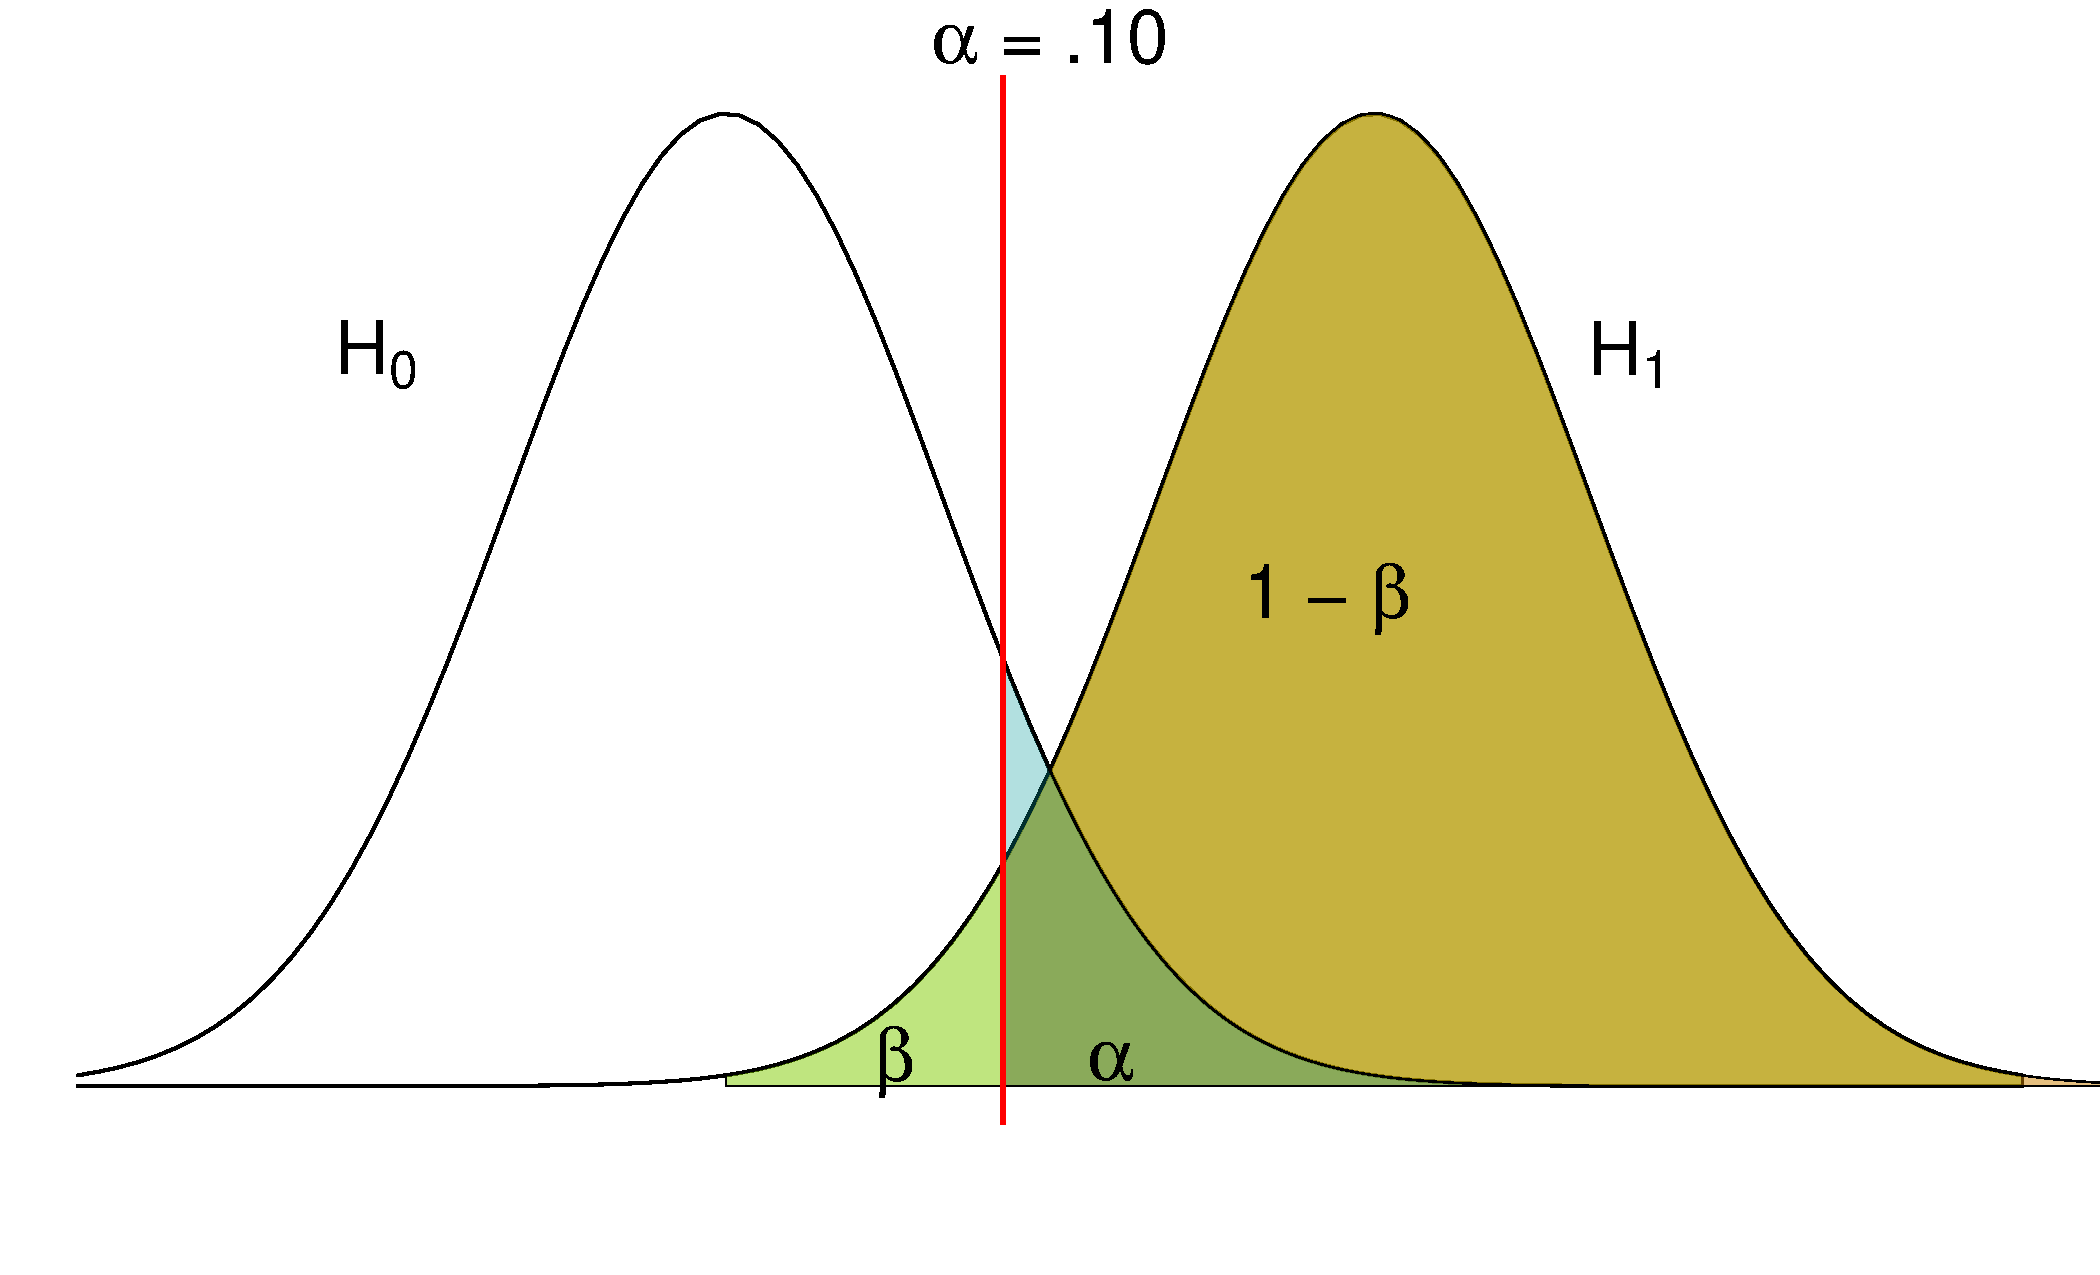
\includegraphics[width=.45\linewidth]{img/power10.pdf}
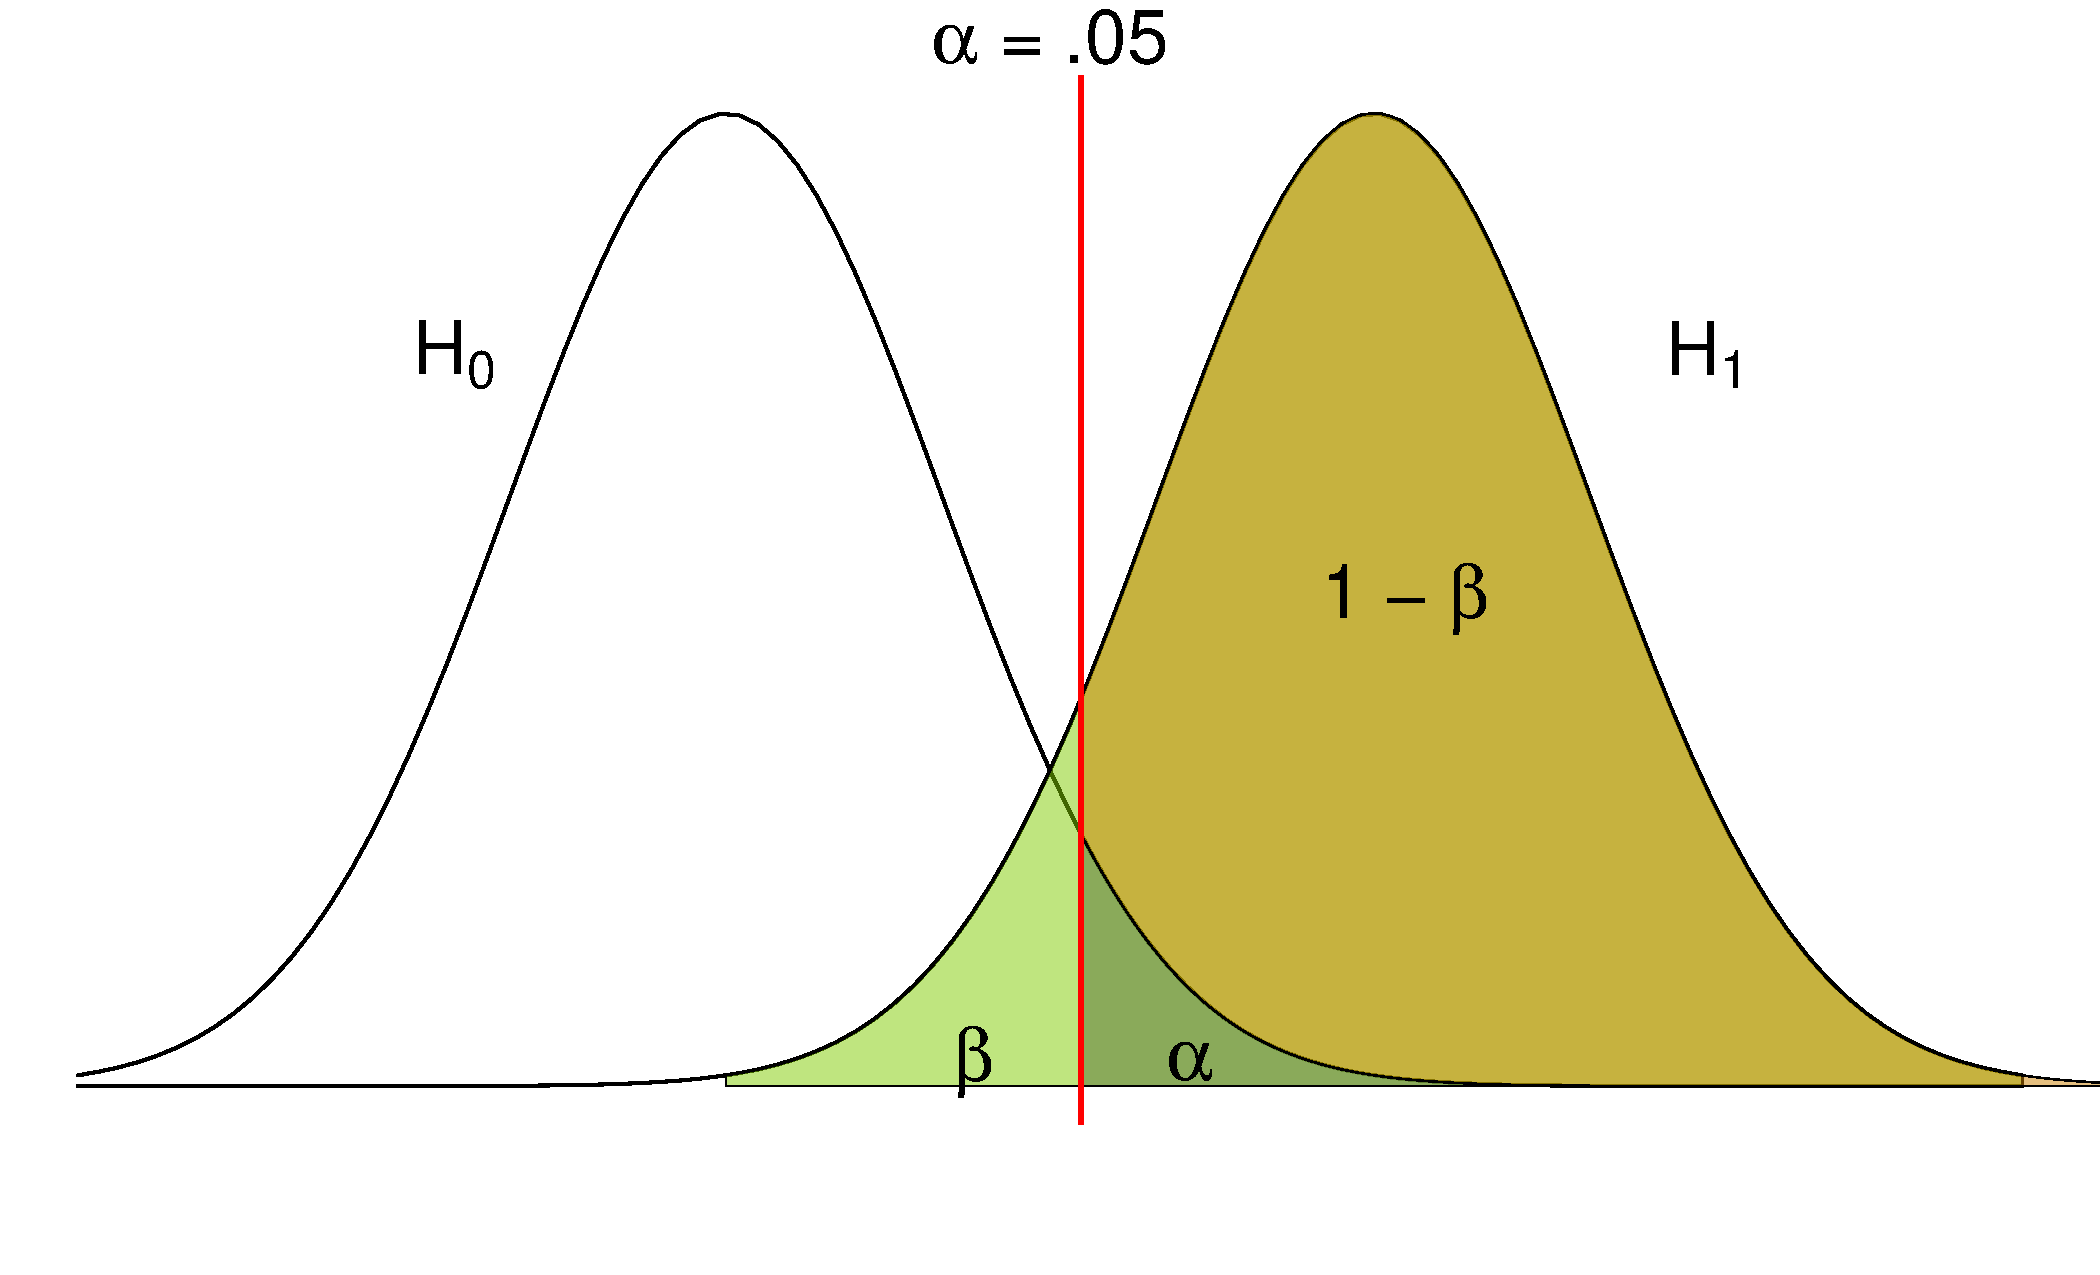
\includegraphics[width=.45\linewidth]{img/power05.pdf}

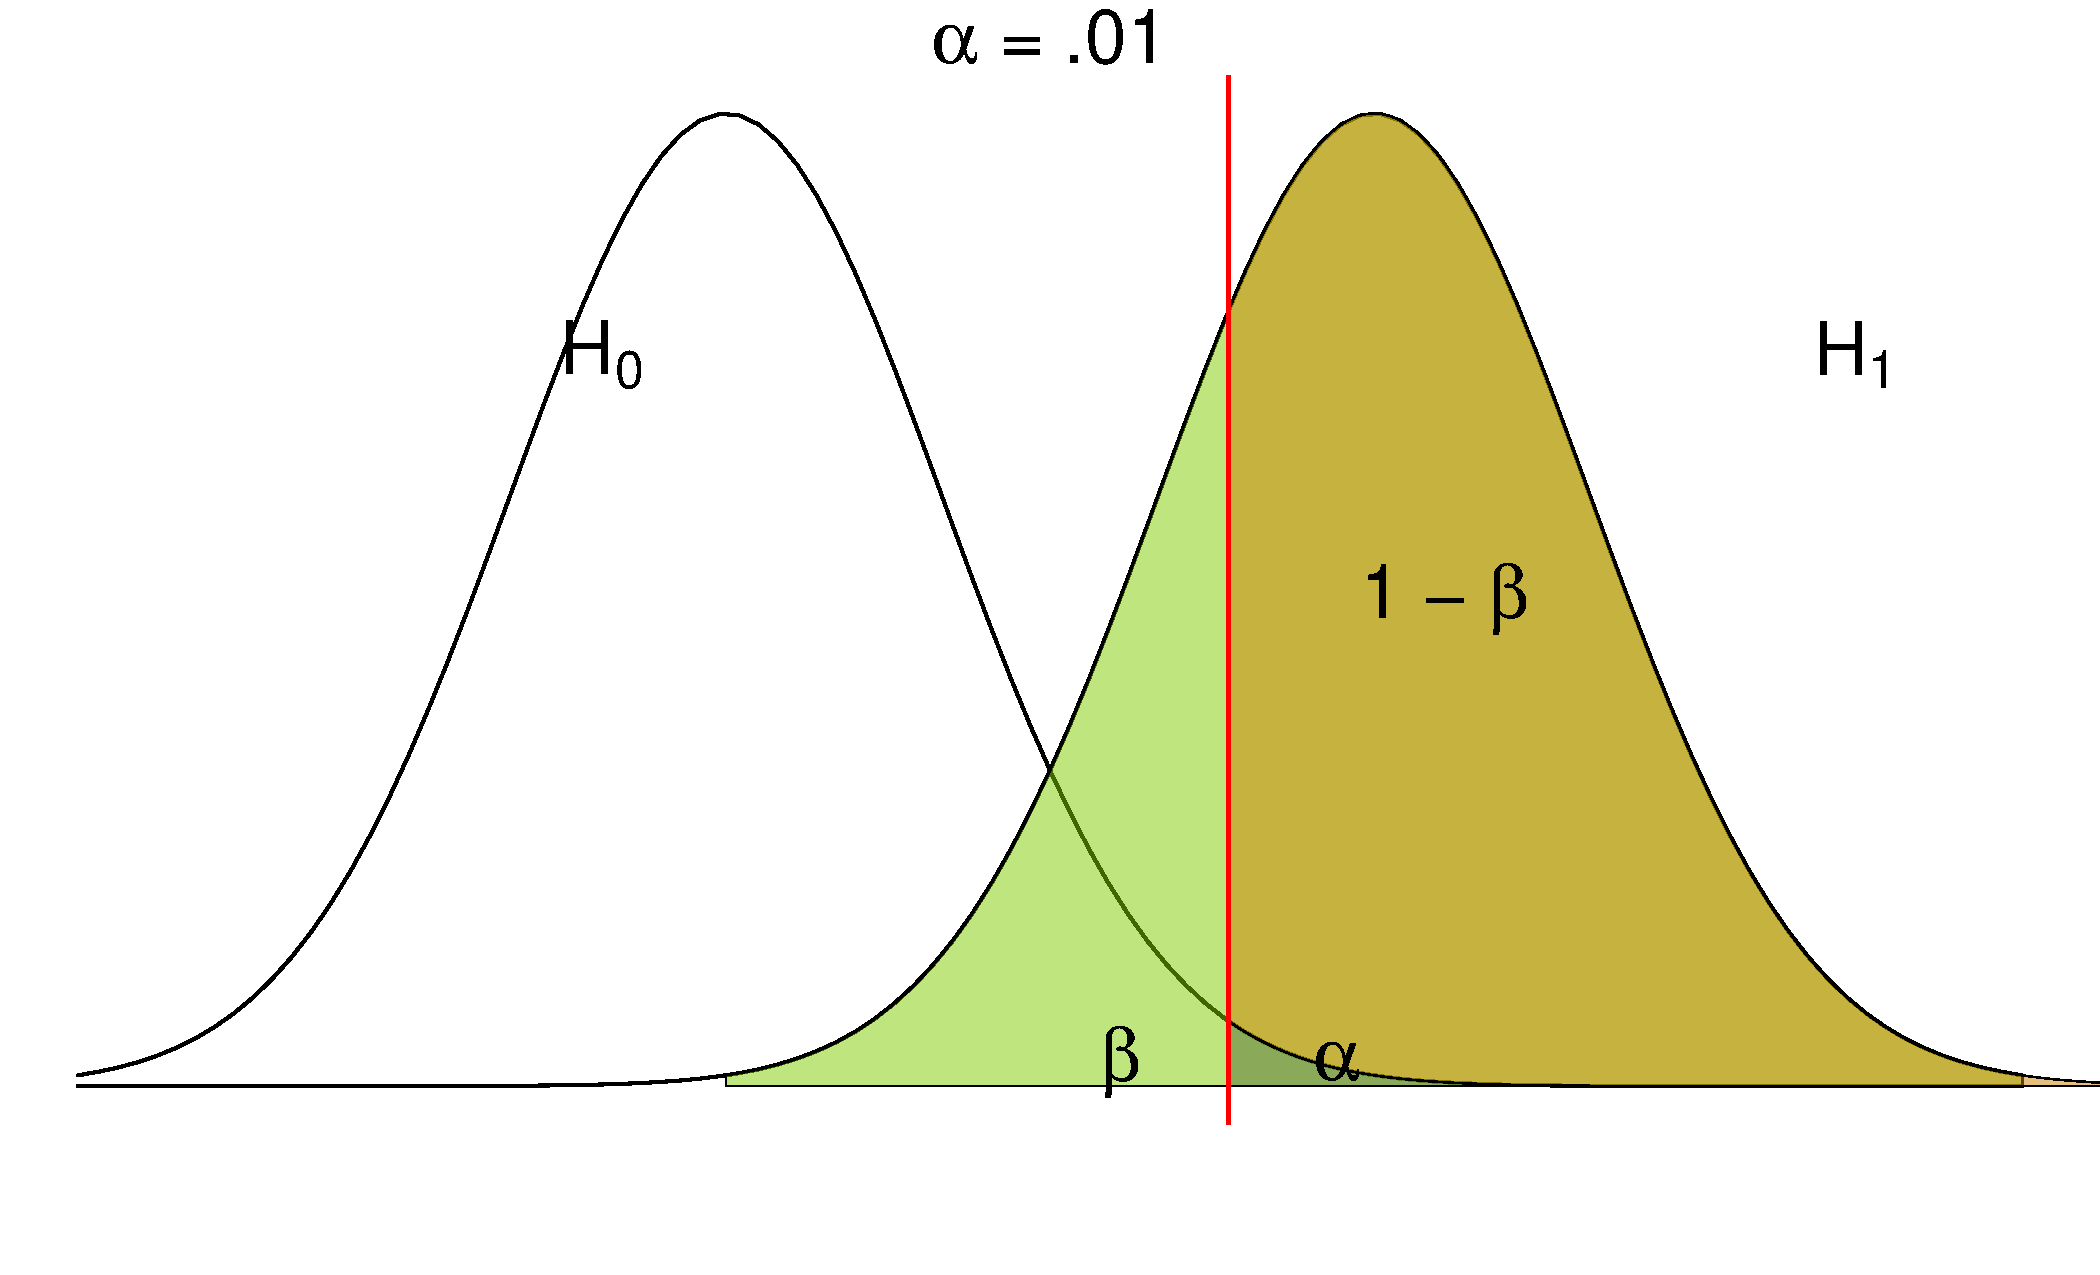
\includegraphics[width=.45\linewidth]{img/power01.pdf}
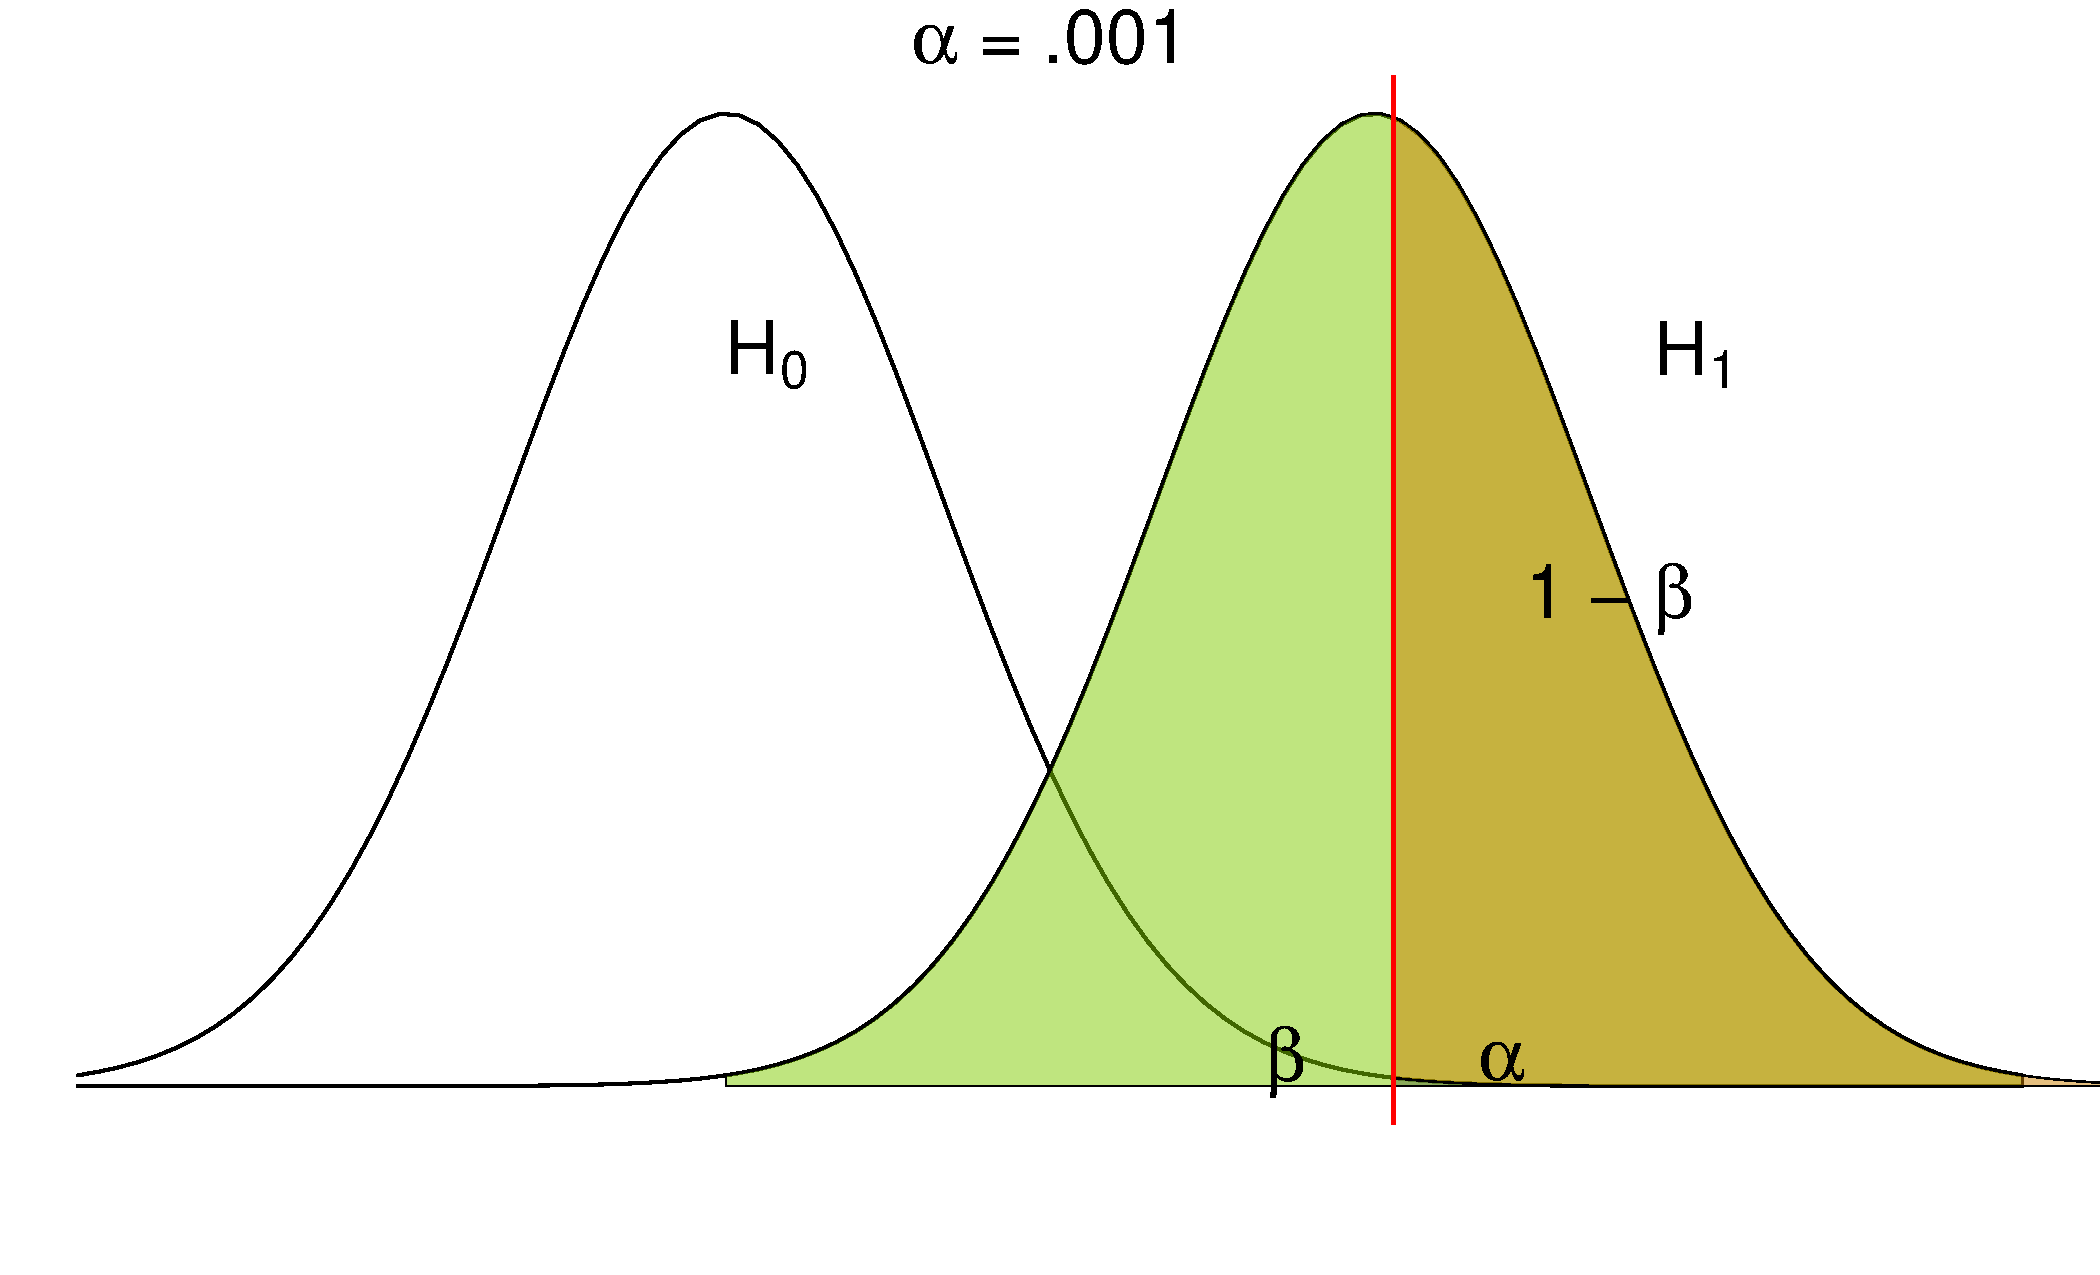
\includegraphics[width=.45\linewidth]{img/power001.pdf}
\end{column}

\begin{column}{0.3\linewidth}
\footnotesize

\begin{longtable}[]{@{}ccc@{}}
\toprule\noalign{}
\(\alpha\) & \(\beta\) & \(1 - \beta\) \\
\midrule\noalign{}
\endhead
.10 & .04 & .96 \\
.05 & .09 & .91 \\
.01 & .25 & .75 \\
.001 & .54 & .46 \\
\bottomrule\noalign{}
\end{longtable}

\vspace{3mm}

\(\mu_0 = 0\), \(\mu_1 = 3\)

\vspace{1mm}

\scriptsize

Bianca: sotto \(H_0\); colorata: sotto \(H_1\) (unilaterale destro)

\vspace{1mm}

Se \(\alpha\) diminuisce, \(\beta\) aumenta e la potenza \(1-\beta\)
diminuisce
\end{column}
\end{columns}
\end{frame}

\subsection{Regola decisionale}\label{regola-decisionale}

\begin{frame}{}
\phantomsection\label{section-24}
\small

\begin{tcolorbox}[enhanced jigsaw, opacityback=0, bottomtitle=1mm, bottomrule=.15mm, titlerule=0mm, coltitle=black, toprule=.15mm, breakable, toptitle=1mm, colbacktitle=quarto-callout-tip-color!10!white, arc=.35mm, title={Valore critico e \(p\)-value}, rightrule=.15mm, leftrule=.75mm, opacitybacktitle=0.6, left=2mm, colframe=quarto-callout-tip-color-frame, colback=white]

In generale, se indichiamo con \(\psi_c\) e \(\psi_o\) rispettivamente
il \textbf{valore critico} e il \textbf{valore osservato} di una
statistica \(\psi\), allora sussiste il seguente rapporto relazionale
tra \((p\text{-value}, \alpha)\) e \((\psi_c, \psi_o)\):

\end{tcolorbox}

\begin{columns}[T]
  \column{0.45\textwidth}
  \centering
  \fbox{
    \begin{minipage}{0.85\textwidth}
      \[
      \begin{aligned}
        p\text{-value} &< \alpha \Rightarrow H_A \\
        p\text{-value} &\geq \alpha \Rightarrow \neg H_A
      \end{aligned}
      \]
    \end{minipage}
  }

  \column{0.1\textwidth}
  \vspace*{5mm}
  \centering
  \Large $\Leftrightarrow$

  \column{0.45\textwidth}
  \centering
  \fbox{
    \begin{minipage}{0.85\textwidth}
      \[
      \begin{aligned}
        \text{Bidir.: } |\psi_o| &> |\psi_c| \Rightarrow H_A \\
        \text{Destra: } \psi_o &> \psi_c \Rightarrow H_A \\
        \text{Sinistra: } \psi_o &< \psi_c \Rightarrow H_A
      \end{aligned}
      \]
    \end{minipage}
  }
\end{columns}

\footnotesize

\begin{tcolorbox}[enhanced jigsaw, opacityback=0, bottomtitle=1mm, bottomrule=.15mm, titlerule=0mm, coltitle=black, toprule=.15mm, breakable, toptitle=1mm, colbacktitle=quarto-callout-important-color!10!white, arc=.35mm, title={Significatività statistica}, rightrule=.15mm, leftrule=.75mm, opacitybacktitle=0.6, left=2mm, colframe=quarto-callout-important-color-frame, colback=white]

\textbf{\underline{Statisticamente significativo}} (si rifiuta \(H_0\)):
\(\psi_o\) cade nella regione di rifiuto definita da \(\psi_c\), cioè
\(p\text{-value} < \alpha\)

\textbf{\underline{Statisticamente non significativo}} (non si rifiuta
\(H_0\)): \(\psi_o\) cade nella regione di non rifiuto, cioè
\(p\text{-value} \geq \alpha\)

\end{tcolorbox}
\end{frame}

\subsection{\texorpdfstring{Cos'è il
\(p\)-value?}{Cos'è il p-value?}}\label{cosuxe8-il-p-value}

\begin{frame}{}
\phantomsection\label{section-25}
\begin{center}
\emph{Il p-value indica la probabilità di osservare un valore uguale o più estremo rispetto a quello osservato, \textbf{posto che sia vera $H_0$}}

\vspace{2mm}

\small
\begin{tabular}{lll}
Unilaterale destro: & $P(T \geq T_0 \mid H_0)$ \\
Unilaterale sinistro: & $P(T \leq T_0 \mid H_0)$ \\
Bidirezionale: & $P(|T| \geq |T_0| \mid H_0)$ \\
\end{tabular}
\end{center}

\begin{tcolorbox}[enhanced jigsaw, opacityback=0, bottomtitle=1mm, bottomrule=.15mm, titlerule=0mm, coltitle=black, toprule=.15mm, breakable, toptitle=1mm, colbacktitle=quarto-callout-note-color!10!white, arc=.35mm, title={Un esempio}, rightrule=.15mm, leftrule=.75mm, opacitybacktitle=0.6, left=2mm, colframe=quarto-callout-note-color-frame, colback=white]

Test bidirezionale, \(T_0 = 2.70\), \(p\)-value = \(.0073\)
(\(p < .01\))

Se \(H_0\) fosse vera e si replicasse l'esperimento moltissime volte,
quante volte si otterrebbe un valore della statistica uguale o più
estremo di \(2.70\)?

\(P(|T| \geq 2.70 \mid H_0) = .0073\): Se fosse vera \(H_0\), il
risultato osservato sarebbe un risultato estremamente poco probabile,
per cui questo risultato si osserverebbe meno dell'1\% delle volte

\end{tcolorbox}
\end{frame}

\begin{frame}{Dettagli sul \(p\)-value}
\phantomsection\label{dettagli-sul-p-value}
\begin{itemize}
\tightlist
\item
  Il \(p\)-value è la probabilità di ottenere un valore uguale o più
  estremo rispetto a \(T_0\) \emph{se \(H_0\) fosse vera}.
  \underline{NON} è la probabilità che \(H_0\) sia vera \(\rightarrow\)
  non può essere usato come indicatore della verità o falsità di \(H_0\)
\item
  Il \(p\)-value è sensibile all'ampiezza campionaria: se \(H_0\) è
  falsa, all'aumentare dell'ampiezza campionaria il \(p\)-value tende a
  diminuire e aumenta la probabilità di rigettare \(H_0\) (anche
  differenze molto piccole diventano significative con campioni grandi).
  Se \(H_0\) è vera, aumentare \(n\) non rende il \(p\)-value più
  piccolo
\item
  Il \(p\)-value permette solo di prendere una decisione qualitativa nei
  termini di ``Non rigetto \(H_0\)'' vs.~``Rigetto \(H_0\)''
  \(\rightarrow\) \textbf{Non è una misura dell'evidenza statistica}
\end{itemize}
\end{frame}

\section{Un esempio completo}\label{un-esempio-completo}

\begin{frame}{La moneta: ipotesi e livello di significatività}
\phantomsection\label{la-moneta-ipotesi-e-livello-di-significativituxe0}
\small

Si lancia la moneta \textbf{30 volte} e si ottengono \textbf{21 teste}.
La moneta è truccata?

\vspace{2mm}

\begin{enumerate}
\item
  \textbf{Ipotesi} (bidirezionale: non si sa in quale direzione potrebbe
  essere truccata) \[H_0: \pi = .50 \qquad H_1: \pi \neq .50\]
\item
  \textbf{Livello di significatività} (fissato prima di lanciare la
  moneta): \(\alpha = .05\)
\item
  \textbf{Statistica}: la proporzione di teste nel campione,
  \(\hat{p} = \frac{21}{30} = .70\)
\end{enumerate}

\vspace{2mm}

\footnotesize

\(\hat{p}\) è una media: se si codifica testa = 1 e croce = 0, la
proporzione di teste è la media dei 30 valori 0/1
\end{frame}

\begin{frame}{La moneta: distribuzione campionaria sotto \(H_0\)}
\phantomsection\label{la-moneta-distribuzione-campionaria-sotto-h_0}
\small

Se \(H_0\) è vera, ogni lancio vale 1 con probabilità \(.50\) e 0 con
probabilità \(.50\): nella ``popolazione'' dei lanci \(\mu = .50\) e
\(\sigma = \sqrt{.50 \times .50} = .50\)

\vspace{2mm}

\begin{enumerate}
\setcounter{enumi}{3}
\tightlist
\item
  \textbf{Distribuzione campionaria} di \(\hat{p}\) sotto \(H_0\):
\end{enumerate}

\begin{itemize}
\tightlist
\item
  centro: \(\mu_{\hat{p}} = .50\)
\item
  errore standard:
  \(\sigma_{\hat{p}} = \frac{\sigma}{\sqrt{n}} = \frac{.50}{\sqrt{30}} = .091\)
\item
  forma: con \(n = 30\) è approssimativamente normale (teorema del
  limite centrale)
\end{itemize}

\vspace{2mm}

\begin{enumerate}
\setcounter{enumi}{4}
\tightlist
\item
  \textbf{Statistica test} (standardizzazione):
  \[z_o = \frac{\hat{p} - \pi_0}{\sigma_{\hat{p}}} = \frac{.70 - .50}{.091} = 2.19\]
\end{enumerate}
\end{frame}

\begin{frame}[fragile]{La moneta: valore critico e \(p\)-value}
\phantomsection\label{la-moneta-valore-critico-e-p-value}
\small

\begin{enumerate}
\setcounter{enumi}{5}
\tightlist
\item
  \textbf{Valore critico}: test bidirezionale con \(\alpha = .05\)
  \(\rightarrow\) \(z_c = \pm 1.96\)
\end{enumerate}

\begin{center}
\begin{tikzpicture}[scale=0.75]
  \fill[unipd!35] (-3.3,0) -- plot[domain=-3.3:-1.96,samples=60] (\x,{2.2*exp(-\x*\x/2)}) -- (-1.96,0) -- cycle;
  \fill[unipd!35] (1.96,0) -- plot[domain=1.96:3.3,samples=60] (\x,{2.2*exp(-\x*\x/2)}) -- (3.3,0) -- cycle;
  \draw[thick] plot[domain=-3.3:3.3,samples=60] (\x,{2.2*exp(-\x*\x/2)});
  \draw (-3.3,0) -- (3.3,0);
  \draw[dashed] (-1.96,0) -- (-1.96,2.4); \node[below, font=\scriptsize] at (-1.96,0) {$-1.96$};
  \draw[dashed] (1.96,0) -- (1.96,2.4); \node[below, font=\scriptsize] at (1.96,0) {$1.96$};
  \draw[very thick, blu, ->] (2.19,2.2) -- (2.19,0.12);
  \node[above, blu, font=\scriptsize] at (2.19,2.2) {$z_o = 2.19$};
  \node[font=\scriptsize] at (0,0.9) {Non rifiuto};
  \node[font=\scriptsize, unipd] at (-2.7,0.9) {Rifiuto};
  \node[font=\scriptsize, unipd] at (2.9,0.9) {Rifiuto};
\end{tikzpicture}
\end{center}

\begin{enumerate}
\setcounter{enumi}{6}
\tightlist
\item
  \textbf{\(p\)-value}:
  \(P(|Z| \geq 2.19 \mid H_0) = 2 \times .014 = .029\)
\end{enumerate}

\begin{Shaded}
\begin{Highlighting}[]
\DecValTok{2} \SpecialCharTok{*}\NormalTok{ (}\DecValTok{1} \SpecialCharTok{{-}} \FunctionTok{pnorm}\NormalTok{(}\FloatTok{2.19}\NormalTok{))   }\CommentTok{\# 0.0285}
\end{Highlighting}
\end{Shaded}
\end{frame}

\begin{frame}[fragile]{La moneta: decisione}
\phantomsection\label{la-moneta-decisione}
\small

\begin{tcolorbox}[enhanced jigsaw, opacityback=0, bottomtitle=1mm, bottomrule=.15mm, titlerule=0mm, coltitle=black, toprule=.15mm, breakable, toptitle=1mm, colbacktitle=quarto-callout-important-color!10!white, arc=.35mm, title={Decisione}, rightrule=.15mm, leftrule=.75mm, opacitybacktitle=0.6, left=2mm, colframe=quarto-callout-important-color-frame, colback=white]

\(|z_o| = 2.19 > 1.96\) e \(p = .029 < .05\) \(\rightarrow\) \textbf{si
rifiuta \(H_0\)}: 21 teste su 30 lanci è un risultato poco compatibile
con una moneta non truccata

\end{tcolorbox}

\vspace{2mm}

\begin{itemize}
\tightlist
\item
  Le due regole (valore critico e \(p\)-value) portano sempre alla
  stessa decisione
\item
  La decisione può essere sbagliata: se la moneta in realtà non fosse
  truccata, si starebbe commettendo un \textbf{errore di I tipo}, la cui
  probabilità è \(\alpha = .05\)
\item
  Con \(\alpha = .01\) (\(z_c = \pm 2.58\)) la decisione sarebbe stata
  diversa: non si rifiuterebbe \(H_0\)
\end{itemize}

\vspace{2mm}

\footnotesize

Con la distribuzione binomiale esatta (\texttt{binom.test(21,\ 30)}) si
ottiene \(p = .043\): la decisione con \(\alpha = .05\) non cambia
\end{frame}




\end{document}
